% ====================================================================
% graphite_ica_ch2_v1.0.15.tex — Chapter 2 (release 1.0.15; 계보 1.0.13 승계 — Fable 전수 재검 반영 —
%   H-1 BW 부호·M-8 파생D 근사 명시·M-9 고온 코너 한정. 계보 v5: 코인 하프셀 엔트로피·가역
%   발열의 통계열역학, Opus build — v4-11 기반, w_eff 절 제거 정정본)
%   ★v5 = intercalation 엔트로피·가역 발열의 *통계열역학 챕터* — 분포를 명시
%        전개(분배함수 Z → 점유 분포 ⟨n⟩ = Ch1 logistic 의 기원 → configurational
%        ·vibrational(BE)·electronic(FD) 엔트로피 → 섞임/겹침 닫힌식(A·B·D)
%        → 극한·코너(I) → 가역 발열 = 분포 재배열 열).
%   ★v5 정정(v4 대비): 파생 C(w_eff(Ω)=w(1-Ω/2RT) "상호작용이 종을 좁힘") 절
%        완전 제거 — two-phase 실측은 *종*이지 델타가 아니라 narrowing 그림이 틀림.
%        대체: w(logistic 폭)는 두-상(Ω>2RT)서 *현상학적 자유 피팅 파라미터*이며,
%        실측 종 폭의 기원(단일입자 율속 꼬리 + 내재 RT/F + 집합 다입자 통계역학
%        apparent-U=U_j+η 앙상블 분포)은 Chapter 1 의 broadening 절 참조.
%        통계열역학 본체(A·B·D, 분배함수→점유분포→S_config·vib·elec·히스)는 보존.
%   범위: 코인 하프셀 단독(단일 전극 vs Li). 전셀 합성(∂U_cell) 범위 외.
%   build: xelatex 2-pass (kotex).
% ====================================================================
\documentclass[11pt,a4paper]{article}
\usepackage[margin=22mm]{geometry}
\usepackage{kotex}
\setmonofont{D2Coding}[Scale=MatchLowercase]
\usepackage{amsmath,amssymb,mathtools,bm}
\usepackage{booktabs,longtable,array}
\usepackage{enumitem}
\usepackage{amsthm}
\usepackage{tikz}
\usetikzlibrary{calc,arrows.meta,decorations.pathreplacing,positioning}
\usepackage{hyperref}
\usepackage{fancyhdr}
\usepackage{lastpage}
\usepackage{setspace}
\setstretch{1.12}
\setlength{\parskip}{0.45em}\setlength{\parindent}{0pt}\setlength{\headheight}{14pt}
\setlength{\emergencystretch}{2em}
\hypersetup{colorlinks=true, linkcolor=blue, urlcolor=blue, citecolor=blue,
  pdftitle={흑연 음극 dQ/dV — Chapter 2 (v1.0.15): 코인 하프셀 엔트로피·가역 발열의 통계열역학}}
\pagestyle{fancy}\fancyhf{}
\lhead{흑연 음극 $dQ/dV$ — Ch.2 (v1.0.15, 엔트로피 통계열역학)}\rhead{\thepage/\pageref{LastPage}}
\renewcommand{\headrulewidth}{0.4pt}
\newtheorem*{keybox}{핵심}
\newtheorem*{srcbox}{문헌 근거}
\newtheorem*{warnbox}{주의}
\newtheorem*{derbox}{유도}
\newtheorem*{procedurebox}{계산 절차}
\newcommand{\dd}{\mathrm{d}}
\newcommand{\rxn}{\mathrm{rxn}}
\newcommand{\eq}{\mathrm{eq}}
\newcommand{\rev}{\mathrm{rev}}
\newcommand{\irr}{\mathrm{irr}}
\newcommand{\oc}{\mathrm{oc}}
\newcommand{\config}{\mathrm{config}}
\newcommand{\vib}{\mathrm{vib}}
\newcommand{\eff}{\mathrm{eff}}
\newcommand{\app}{\mathrm{app}}
\newcommand{\hys}{\mathrm{hys}}
\newcommand{\cell}{\mathrm{cell}}
\newcommand{\kB}{k_{\mathrm B}}
\newcommand{\avg}[1]{\langle #1\rangle}
\renewcommand{\theequation}{2.\arabic{equation}}
\renewcommand{\thesection}{2.\arabic{section}}
\title{\textbf{\LARGE Chapter 2}\\[0.35em]\Large 코인 하프셀 엔트로피와 가역 발열의 통계열역학\\[0.2em]\large — 분배함수에서 점유 분포로, 분포에서 $\partial U/\partial T\cdot\Delta S(x)\cdot\dot Q_\rev$ 로}
\author{}\date{}

\begin{document}
\maketitle

% ====================================================================
\section*{서 — 왜 엔트로피에는 통계가 필요한가}
\addcontentsline{toc}{section}{서}
% ====================================================================
Chapter 1 은 흑연 음극의 한 $\dd Q/\dd V$ 곡선을, 전이별 평형 중심 전위
$U_j(T)=(-\Delta H_{\rxn,j}+T\,\Delta S_{\rxn,j})/F$ 위에 세운 평형 종과 그 위에 얹힌 동역학 꼬리로
설명했다. 그 곡선의 평형 골격에는 이미 한 가지 ``열''이 잠겨 있다. 평형 중심의 \emph{온도 의존}
$\partial U_j/\partial T$ 인데, 열역학 1$\cdot$2법칙은 이 기울기를 곧장 반응 엔트로피로 환산한다. 그리고
반응 엔트로피야말로 전지가 충방전하며 흡수$\cdot$방출하는 \emph{가역(엔트로피) 발열}의 원천이다. 본 장의
일은 이 잠긴 열을 끄집어내어 정량화하는 것이다.

문제는, 엔트로피를 ``$\partial U/\partial T$ 를 측정하면 나오는 수''로만 다루면 그 \emph{모양}을 이해할 수
없다는 데 있다. 흑연 하프셀의 측정 엔트로피 계수 $\partial U_\oc/\partial T(x)$ 는 SOC(state of charge)에 따라 부호를 바꾸고
($x$ 작을 때 양, 클 때 음), 전이 경계마다 봉우리와 골을 만들며, 어떤 자리에서는 발산에 가깝게 치솟는다. 이
비선형 모양을 ``전이마다 상수 $\Delta S_{\rxn,j}$ 를 가정''하는 평형 정전 식만으로는 재현하지 못한다. 모양은
\emph{분포}에서 온다 — Li 이온이 격자 자리들에 \emph{어떻게 흩어져 앉아 있는가}, 격자 진동이 포논 모드에
\emph{어떻게 분배되는가}, 전도 전자가 Fermi 준위 부근에 \emph{어떻게 채워지는가}. 엔트로피는 본질적으로
이 미시상태 분포의 흩어짐 척도이고, 가역 발열
\[
\dot Q_\rev=-I\,T\,\frac{\partial U_\oc}{\partial T}=-\frac{I\,T}{F}\,\Delta S(x)
\]
은 한 충전상태에서 다른 충전상태로 넘어갈 때 \emph{이 분포를 재배열하면서 주고받는 열}이다. 곧
$\partial U_\oc/\partial T(x)$ 의 모양을 이해하려면, 그 밑에 깔린 점유 분포를 명시적으로 세워야 한다.

이에 본 장은 통계열역학 챕터로 구성한다. 분포를 결론으로 인용하는 대신 \emph{본체}로 전개한다. 출발점은 단일 격자
자리의 분배함수 $Z$ 이고(\S\ref{sec:partition}), 거기서 점유 분포 $\avg{n}$ 을 얻는데 이것이 바로 Chapter 1
의 logistic 평형 점유의 통계역학적 기원임을 보인다. 점유 분포에서 Boltzmann--Shannon 엔트로피
$S_\config=-R\sum p\ln p$ 가 나오고(\S\ref{sec:config}), 같은 분포 언어로 격자 진동(포논 Bose--Einstein)과
전도 전자(Fermi--Dirac)의 엔트로피를 더한다(\S\ref{sec:vibel}). 세 분포가 합쳐져 측정 $\partial U_\oc/\partial T(x)$
의 모든 모양 — 봉우리 겹침, 봉우리 내부 발산, 히스테리시스 분기 — 을 만든다
(\S\ref{sec:mixing}). 극한과 코너(corner case — 경계$\cdot$예외 상황)에서 검산하고(\S\ref{sec:limits}), 마지막으로 분포 재배열로서의 가역
발열로 닫는다(\S\ref{sec:revheat}). 사슬은
\[
\boxed{\;Z \;\to\; \avg{n}=\text{점유 분포}\;\to\; S=-R\textstyle\sum p\ln p \;\to\; \frac{\partial U_\oc}{\partial T}(x)=\frac{\Delta S(x)}{F}\;\to\;\dot Q_\rev=-I\,T\,\frac{\partial U_\oc}{\partial T}\;}
\]
이고, 각 화살표는 점프 없이 분포에서 유도된다.

\begin{warnbox}
\textbf{범위 — 코인 하프셀 단독.} 본 장은 단일 전극(흑연 vs.\ Li 금속)의 하프셀 $\partial U_\oc/\partial T$ 와
그 가역 발열만 다룬다. 전셀 합성 $\partial U_\mathrm{cell}/\partial T=\partial U_\mathrm{cat}/\partial T-\partial
U_\mathrm{an}/\partial T$ (양극$-$음극 차감)는 \emph{범위 밖}이다 — 본 장의 분포는 한 전극의 점유 분포다.
주 사례는 흑연 음극 하프셀이며, LCO 의 전자 엔트로피 항은 분포 언어의 한 사례로만 포함한다.
\end{warnbox}

% ====================================================================
\section{격자기체 분배함수에서 점유 분포로}\label{sec:partition}
% ====================================================================
통계역학에서 한 계의 모든 평형 열역학량은 분배함수에서 나온다. 흑연 격자에 Li 이온이 삽입되는 문제는
\emph{격자기체}(lattice gas)로 모형화된다 \cite{newman,huggins2009}: 결정 안에 동등한 삽입 자리들이 있고,
각 자리는 비어 있거나(에너지 0) Li 하나가 점유한다(에너지 $\varepsilon_0$). 자리들은 전해질을 통해 Li 저장조
(상대극 Li 금속)와 평형을 이루므로 전기화학 퍼텐셜 $\mu$ 가 고정된 \emph{대정준}(grand-canonical) 문제다.
이 절은 그 분배함수를 세우고, 거기서 점유 분포 $\avg{n}$ 을 끌어낸 뒤, 그것이 Chapter 1 이 \emph{이미 쓰고
있던} logistic 평형 점유의 기원임을 보이고, 자리 사이 상호작용을 켠 다자리 평균장(Bragg--Williams,
\S\ref{ssec:BW})으로 절을 닫는다. 이 유도의 통계역학 배경(ensemble$\cdot$Gibbs 인자$\cdot$화학퍼텐셜
$\mu$ 의 의미)은 Chapter 1 의 Part 0(통계역학 기초)이 처음부터 자세히 세웠다 — 여기서는 발열 논의에 필요한
최소 사슬만 자기완결로 다시 놓는다.

\subsection{단일 자리 대정준 분배함수}
자리 하나를 분리하여 살펴본다. 두 미시상태 — 빈 자리($n=0$, 에너지 0)와 점유($n=1$, 에너지 $\varepsilon_0$) — 의
대정준 분배함수는 각 상태에 Gibbs 인자 $e^{-\beta(\varepsilon_0-\mu)n}$ 을 곱해 더한 것이다($\beta=1/\kB T$):
\begin{equation}
\Xi_1 \;=\; \sum_{n=0,1} e^{-\beta(\varepsilon_0-\mu)\,n}
\;=\; 1 \;+\; e^{-\beta(\varepsilon_0-\mu)}.
\label{eq:Z1}
\end{equation}
자리의 평균 점유는 정의상 분배함수의 로그 미분, 곧 두 상태의 확률 가중 평균이다:
\begin{equation}
\avg{n} \;=\; \frac{0\cdot 1 + 1\cdot e^{-\beta(\varepsilon_0-\mu)}}{\Xi_1}
\;=\; \frac{e^{-\beta(\varepsilon_0-\mu)}}{1+e^{-\beta(\varepsilon_0-\mu)}}
\;=\; \frac{1}{1+e^{\beta(\varepsilon_0-\mu)}}.
\label{eq:occ}
\end{equation}
이 $\avg{n}$ 은 자리가 채워질 확률 $p_1$ 그 자체이고, 빌 확률은 $p_0=1-\avg{n}$ 이다. 식~\eqref{eq:occ} 는
구조상 \emph{Fermi--Dirac 함수}와 동형이다 — 자리당 2-상태(채움/빔)가 전자 준위의 점유/공위와 같은
대수 구조를 낳으며, 다른 점은 ``입자''가 페르미온 전자가 아니라 Li 이온이고 단일 준위 에너지가
$\varepsilon_0-\mu$ 라는 것뿐이다. 기호와 엄밀성에 관한 두 가지를 밝혀 둔다. 첫째, $\Xi_1$ 은 자리 1개의
\emph{대정준} 분배함수이며 Chapter 1 Part 0 의 같은 기호와 통일한 표기다(canonical 분배함수와 기호부터
구분). 둘째, 점유된 이온이 자리 우물 안에서 갖는 진동 등 내부 자유도의 분배함수 $q(T)$ 까지 포함한 엄밀
유도는 Chapter 1 Part 0 이 닫았다 — 그 결과는 $\varepsilon_0$ 을 유효 자리 자유에너지
$\tilde\varepsilon=\varepsilon_0-\kB T\ln q(T)$ 로 대체하는 것뿐이고 logistic 함수형은 불변이므로, 본 장
이하의 $\varepsilon_0$ 은 그 흡수를 마친 유효값으로 읽는다. 그 내부 자유도의 온도 미분이
\S\ref{sec:vibel} 의 vibrational 엔트로피 몫의 단일 자리 원형이다.

\subsection{전기화학 퍼텐셜과 Chapter 1 logistic 의 기원}\label{ssec:logistic}
이제 화학을 넣는다. Li 가 자리에 들어가는 전기화학 반응의 전기화학 퍼텐셜은 셀 전위에 선형으로 묶인다:
\begin{equation}
\mu \;=\; \mu^0 \;-\; s\,F\,(V-U_j),
\label{eq:muV}
\end{equation}
여기서 $V$ 는 (평형) 전극 전위, $U_j$ 는 그 전이의 표준(중심) 전위, $F$ 는 Faraday 상수, $s(=+1)$ 는
Chapter 1 의 \emph{유도 전용 고정 부호}다.\footnote{방향 부호 $\sigma_d$(Chapter 1 — 분극$\cdot$분기$\cdot$꼬리
세 작용처 전용, $\pm1$)와는 별개다 — 평형 관계에는 항상 $s{=}+1$ 이 들어가며, $\sigma_d{=}-1$ 을 이 식에
기계 대입하면 점유와 진행률이 뒤바뀌는 여집합 오류가 생긴다(종은 불변이라 잠복).} 전위가 오르면 ($V>U_j$)
Li 의 전기화학 퍼텐셜이 낮아져 자리에서
빠져나가므로 \emph{점유} $\avg{n}=\theta$ 는 $V$ 에 따라 \emph{감소}한다. 식~\eqref{eq:muV} 를
\eqref{eq:occ} 에 대입하고 $N_A\varepsilon_0\equiv\mu^0$(자리당 값의 몰 환산이 기준 화학퍼텐셜과
일치하는 전이 중심 기준)을 잡으면, 평형 점유와 그
여집합(탈리튬화 진행률 $\xi\equiv1-\theta$)은
\begin{equation}
\boxed{\;\theta_\eq(V,T)=\avg{n}=\frac{1}{1+\exp\!\bigl[+(V-U_j)/w\bigr]},\qquad
\xi_\eq(V,T)=1-\theta_\eq=\frac{1}{1+\exp\!\bigl[-(V-U_j)/w\bigr]}\;,}
\label{eq:logistic}
\end{equation}
이고 여기서 $w\equiv RT/F$ 다. 몰 단위 환산 $R=N_A\kB$, $F=N_Ae$ 로 $\beta(\varepsilon_0-\mu)$ 의 분자를
몰 에너지로 쓰면 지수는 $(V-U_j)/(RT/F)=(V-U_j)/w$, 곧 몰 척도에서 $F/RT=1/w$ 이고 자리당
$\beta=1/\kB T$ 그대로는 $\beta F=N_A/w$ 다. 곧 \emph{점유} $\theta$ 는 $V$ 에
감소하는 logistic, \emph{탈리튬화 진행률} $\xi=1-\theta$ 는 $V$ 에 증가하는 logistic이며, 후자가 정확히
Chapter 1 의 전이별 \emph{logistic 평형 종}이다($\xi\to1$ 고전위$\cdot$Li 희박, $\xi\to0$ 저전위$\cdot$만충).

\begin{keybox}
Chapter 1 의 평형 종 $\xi_\eq$ 는 \emph{현상학적 곡선맞춤}이 아니라 \emph{격자기체 점유 분포의 여집합}(탈리튬화
진행률 $=1-\theta$)이다. logistic 폭 $w=RT/F$($n_j{=}1$ 서식; 일반형 $w_j=n_jRT/F$)는 \emph{단상
전이($\Omega_j\le2RT$)에 한해} 평형 등온선이 정하는 검증 가능한 평형 예측이고(이상 극한은 단일 자리
분배함수~\eqref{eq:Z1} 의 $RT/F$, 상호작용이 있으면 $\Omega$ 가 폭을 바꾸되 그 값 역시 평형 등온선이
결정한다 — \S\ref{ssec:weff}),
\emph{두-상 전이}($\Omega_j>2RT$ — 흑연 staging 의 $2\mathrm L\!\to\!2\cdot2\!\to\!1$)에는 이 유도가 닿지
않아 폭은 현상학적 자유 피팅 파라미터가 된다. 값과 $T$-의존 함수형의 두 층위 구분, 그리고 함수형을 유지할지는 두-상 폭의 모델 선택 문제이며 파생
C(\S\ref{ssec:weff})와 파생 A 전제 명시(\S\ref{ssec:overlap})가 다룬다. ★표기: $\theta=$ Li 점유율(만충에서 1), $\xi=1-\theta=$ 탈리튬화 진행률(희박에서 1); 둘은 같은 점유
분포의 두 이름이다. Chapter 2 는 이 분포를 결론이 아니라 출발점으로 삼아 엔트로피를 쌓는다.
\end{keybox}

$\xi=1-\theta$ 와 전위의 관계를 뒤집으면(점유 $\theta$ 의 Nernst 관계 $V=U_j+(RT/F)\ln[(1-\theta)/\theta]$ 에
$\theta=1-\xi$ 대입)
\begin{equation}
V(\xi) \;=\; U_j \;+\; \frac{RT}{F}\,\ln\!\frac{\xi}{1-\xi},
\label{eq:Vxi}
\end{equation}
이 되는데, 이 \emph{Nernst 형 로그항}이 뒤에서 configurational 엔트로피의 부분몰 형태로 다시 나타난다
(\S\ref{sec:config}). 식~\eqref{eq:Vxi} 의 $\ln[\xi/(1-\xi)]$ 가 단순한 곡선맞춤이 아니라 점유 분포의
엔트로피에서 온다는 것이 이 장의 첫 매듭이다.

\subsection{다자리 평균장 — Bragg--Williams 와 상호작용}\label{ssec:BW}
실제 격자에서는 자리들이 독립이 아니다. 점유된 이웃 자리는 다음 Li 의 삽입 에너지를 바꾼다(정전 반발,
탄성 변형, 전자 구조 변화). 이 상호작용을 평균장으로 다루는 것이 Bragg--Williams 근사다 \cite{huggins2009,
bazant2013}. 점유율 $\theta\in[0,1]$ (자리당 평균 점유, 거시적으로 $\avg{n}$ 과 같음) 의 자유에너지는
\begin{equation}
g(\theta) \;=\; g_0 \;+\; RT\bigl[\theta\ln\theta + (1-\theta)\ln(1-\theta)\bigr]
\;+\; \Omega\,\theta(1-\theta),
\label{eq:BW}
\end{equation}
이고, 우변 둘째 항이 \emph{혼합(섞임) 엔트로피}(곧 \S\ref{sec:config}; Chapter 1 Part 0 의 ``섞임''과 같은 양), 셋째 항이 regular-solution 형 \emph{혼합
엔탈피}다 — 상호작용 모수 $\Omega>0$ 은 같은 종끼리 뭉치려는 인력(상분리 경향), $\Omega<0$ 은
교대 정렬(규칙화) 경향을 뜻한다. 평형 전위는 $\theta$ 1몰 삽입당 자유에너지 변화이므로
\begin{equation}
V_\eq(\theta) \;=\; U_j \;-\; \frac{RT}{F}\ln\!\frac{\theta}{1-\theta} \;-\; \frac{\Omega}{F}\,(1-2\theta),
\label{eq:Veq_BW}
\end{equation}
가 되어, 식~\eqref{eq:Vxi} 의 이상 격자기체에 상호작용 항 $-\Omega(1-2\theta)/F$ 가 더해진다. 이 상호작용의
\emph{열역학적} 결과는 상분리 임계다: $\Omega$ 가 임계값을 넘으면 평형 등온선이 비단조가 되어 분포가 쌍봉
(bimodal)으로 갈리며 \emph{상분리}(plateau)가 일어난다. 임계 조건은 $\partial V_\eq/\partial\theta=0$ 의 첫 등장, 곧
\begin{equation}
\frac{\dd V_\eq}{\dd\theta} \;=\; -\frac{RT}{F}\frac{1}{\theta(1-\theta)} \;+\; \frac{2\Omega}{F},
\qquad
\theta=\tfrac12\text{ 에서 }\;\frac{\dd V_\eq}{\dd\theta}\Big|_{1/2}=\frac{2\Omega-4RT}{F},
\label{eq:slope_BW}
\end{equation}
이 0 이 되는 $\Omega=2RT$ 다. $\Omega\le2RT$ 면 등온선이 단조(균질 고용체 — 등호에선 중심 기울기 0), $\Omega>2RT$ 면 중앙에서
기울기가 양으로 뒤집혀(불안정) 상분리한다. 이 임계 $\Omega=2RT$ 가 \S\ref{sec:limits} 에서 핵심 코너로 다시
나온다.

% ====================================================================
\section{점유 분포에서 configurational 엔트로피로}\label{sec:config}
% ====================================================================
이제 분포에서 엔트로피를 끌어낸다. 한 자리가 점유될 확률 $\theta$, 빌 확률 $1-\theta$ 인 베르누이 분포의
정보 엔트로피(Boltzmann--Shannon 엔트로피)는, 자리 1몰당
\begin{equation}
\boxed{\;S_\config \;=\; -R\sum_i p_i\ln p_i
\;=\; -R\bigl[\theta\ln\theta + (1-\theta)\ln(1-\theta)\bigr]\;.}
\label{eq:Sconfig}
\end{equation}
이것은 Bragg--Williams 자유에너지~\eqref{eq:BW} 의 둘째 항을 $-T$ 로 나눈 것과 정확히 일치한다($g$ 의 엔트로피
부분 $=-T S_\config$). 곧 \S\ref{ssec:BW} 에서 자유에너지로 도입한 혼합 항이, 점유 분포의 엔트로피로서
독립적으로 유도된다 — 자유에너지 모형과 분포 통계가 같은 식으로 만나는 지점이다.

\subsection{부분몰 configurational 엔트로피 — 발산하는 봉우리 내부 항}
가역 발열에 들어가는 것은 \emph{Li 1몰 삽입당} 엔트로피 변화, 곧 부분몰량이다. 식~\eqref{eq:Sconfig} 를
$\theta$ 로 미분하면
\begin{equation}
\frac{\partial S_\config}{\partial\theta}
\;=\; -R\bigl[\ln\theta + 1 - \ln(1-\theta) - 1\bigr]
\;=\; -R\,\ln\!\frac{\theta}{1-\theta},
\label{eq:dSconfig}
\end{equation}
가 되는데, 이것이 이 장의 중심 결과 중 하나다. 식~\eqref{eq:dSconfig} 와 식~\eqref{eq:Vxi} 의 logistic
역함수를 나란히 두면,
\begin{equation}
V(\xi)=U_j+\frac{RT}{F}\ln\!\frac{\xi}{1-\xi}
\;\Longrightarrow\;
\frac{\partial V}{\partial T}\Big|_\xi
= \frac{\Delta S_{\rxn,j}}{F}\;+\;\frac{R}{F}\ln\!\frac{\xi}{1-\xi}
= \frac{\Delta S_{\rxn,j}}{F}\;+\;\frac{1}{F}\frac{\partial S_\config}{\partial\theta}\Big|_{\theta=1-\xi},
\label{eq:dVdT_config}
\end{equation}
임을 확인한다. 첫 항은 $\partial U_j/\partial T=\Delta S_{\rxn,j}/F$ 이고, 둘째 항은 $w=RT/F$ 의 명시적 $T$
의존이 낳는다 — 점유 $\theta=1-\xi$ 에서 $\partial S_\config/\partial\theta|_{\theta=1-\xi}=-R\ln[(1-\xi)/\xi]
=+R\ln[\xi/(1-\xi)]$ 이고, Li 삽입이 점유를 늘리는 방향이라 부호가 $+$ 로 맞물린다. 계수 $R/F$ 는 자리당
$n_j{=}1$ 서식이며 전이별 일반형은 $n_jR/F$ 다(후술 \S\ref{ssec:overlap} 식~\eqref{eq:dxidT}). 곧 \textbf{Chapter 1 의
logistic 폭 $w=RT/F$ 가 이미 부분몰 configurational 엔트로피를 담고 있었다}. 봉우리 내부 $\partial U_\oc/\partial T(x)$
의 $x$-의존(비선형 모양)은 새 물리가 아니라, 점유 분포의 엔트로피가 $w$ 의 온도 의존을 통해 자동으로 들어온 것이다.

부호는 명확하다(그림~\ref{fig:occ_config}; 규약: $\xi$ = 탈리튬화 진행률, $\xi\to1$ = Li 희박, $\xi\to0$ = 만충):
\begin{itemize}[leftmargin=1.4em,itemsep=1pt]
\item $\xi\to1$ (희박, Li-poor): $\ln[\xi/(1-\xi)]\to+\infty$ — config 부분몰 엔트로피 $\to+\infty$. 희박
한계에서 한 Li 를 더 넣을 자리의 \emph{선택지}가 폭증하므로 엔트로피가 발산한다. 저-$x$ 에서
관측되는 큰 양의 $\Delta S$($+29$ J\,mol$^{-1}$K$^{-1}$ 급)는 모델 분해로는 이 분포(config) 발산 몫과
전이 중심 표준값 몫이 나눠 담당한다(귀속의 정량 한정은 표~\ref{tab:ds} 도입 문단) — dilute 격자기체 모형이 같은
발산을 예측한다 \cite{occupation2019}(방법 수준$\cdot$dilute 격자기체 한정 참조).
\item $\xi\to0$ (만충, Li-rich): $\ln[\xi/(1-\xi)]\to-\infty$ — config 부분몰 엔트로피 $\to-\infty$. 거의 다 찬
격자에 마지막 Li 를 끼우면 배열 선택지가 사라져 엔트로피가 음으로 발산한다.
\item $\xi=\tfrac12$ (중심): $\ln 1=0$ — config 기여 $=0$. 봉우리 중심에서 부분몰 config 엔트로피가 정확히
사라지고, $\partial V/\partial T$ 는 표준값 $\Delta S_{\rxn,j}/F$ 로 환원된다.
\end{itemize}

\begin{figure}[t]
\centering
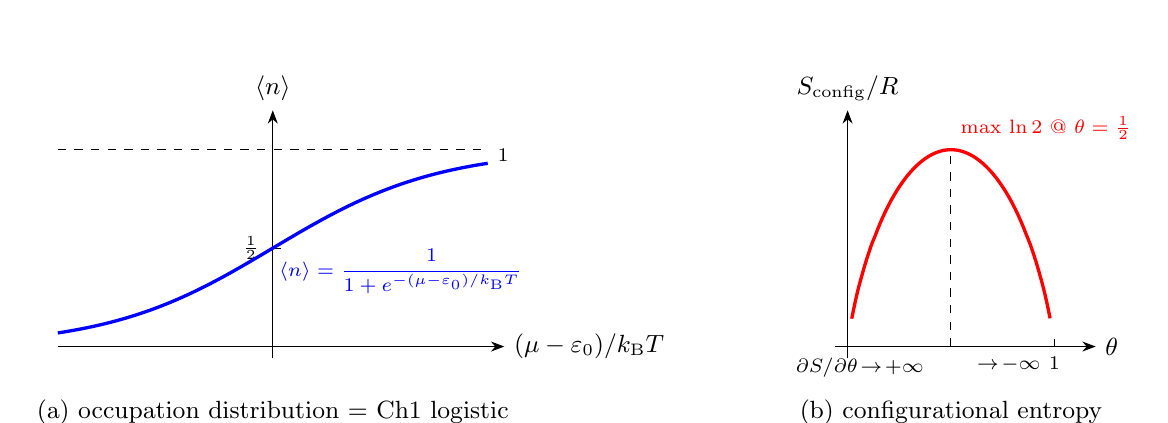
\begin{tikzpicture}[x=1.05cm,y=1.0cm]
% ---- left panel: occupation distribution <n>(eta) ----
\begin{scope}
  \draw[->,>=Stealth] (-2.6,0) -- (2.8,0) node[right]{\small $(\mu-\varepsilon_0)/\kB T$};
  \draw[->,>=Stealth] (0,-0.15) -- (0,3.0) node[above]{\small $\langle n\rangle$};
  \draw[dashed] (-2.6,2.5) -- (2.6,2.5) node[right,yshift=-2pt]{\scriptsize $1$};
  \draw[dashed] (0,1.25) -- (0.12,1.25); \node[left] at (-0.05,1.25){\scriptsize $\tfrac12$};
  % logistic curve n = 1/(1+e^{-eta}), scaled to height 2.5
  \draw[very thick,blue] plot[smooth,domain=-2.6:2.6,samples=60]
    (\x, {2.5/(1+exp(-\x))});
  \node[blue] at (1.55,0.95) {\scriptsize $\langle n\rangle=\dfrac{1}{1+e^{-(\mu-\varepsilon_0)/\kB T}}$};
  \node[below] at (0,-0.55) {\small (a) occupation distribution = Ch1 logistic};
\end{scope}
% ---- right panel: S_config(theta) ----
\begin{scope}[xshift=7.3cm]
  \draw[->,>=Stealth] (-0.15,0) -- (3.0,0) node[right]{\small $\theta$};
  \draw[->,>=Stealth] (0,-0.15) -- (0,3.0) node[above]{\small $S_\mathrm{config}/R$};
  \draw[dashed] (2.5,0) -- (2.5,0.1) node[below,yshift=-3pt]{\scriptsize $1$};
  % S = -[theta ln theta + (1-theta) ln(1-theta)], max ln2~0.693 at 0.5; x:theta*2.5, y: S/0.693*2.5
  \draw[very thick,red] plot[smooth,domain=0.02:0.98,samples=60]
    (\x*2.5, {(-(\x*ln(\x)+(1-\x)*ln(1-\x)))/0.6931*2.5});
  \draw[dashed] (1.25,0) -- (1.25,2.5);
  \node[red,above right] at (1.25,2.5) {\scriptsize max $\ln 2$ @ $\theta=\tfrac12$};
  % partial molar arrows (diverging)
  \node[below] at (0.15,-0.02) {\scriptsize $\partial S/\partial\theta\!\to\!+\infty$};
  \node[below] at (1.95,-0.02) {\scriptsize $\to\!-\infty$};
  \node[below] at (1.25,-0.55) {\small (b) configurational entropy};
\end{scope}
\end{tikzpicture}
\caption{(a) 단일 자리 점유 분포 $\langle n\rangle$~\eqref{eq:occ} — Fermi--Dirac 와 동형이며 Chapter 1 logistic 평형 점유의 기원. (b) configurational 엔트로피 $S_\config(\theta)$~\eqref{eq:Sconfig}; 중심 $\theta=\tfrac12$ 에서 최대 $\ln 2$, 부분몰 $\partial S_\config/\partial\theta=-R\ln[\theta/(1-\theta)]$ 가 양 끝에서 $\pm\infty$ 로 발산(봉우리 내부 $\partial U_\oc/\partial T$ 의 분포 항).}
\label{fig:occ_config}
\end{figure}

\begin{warnbox}
\textbf{이중계산 금지 (파생 B).} 먼저 표기를 고정한다: \textbf{전이 중심 표준 반응 엔트로피}를
$\Delta S^0_j\equiv\Delta S_{\rxn,j}\equiv[\Delta S(x)]_{\xi=1/2}$ 로 한 기호로 정의한다(봉우리 중심 $\xi=\tfrac12$
에서 측정되는 값, config$=0$). 식~\eqref{eq:dVdT_config} 의 두 항은 \emph{서로 다른 출처}이며 한 번씩만 센다.
첫 항 $\Delta S^0_j$ 는 중심 표준값으로 vibrational$\cdot$electronic 의 중심 기여를 이미 흡수한 상수다. 둘째 항
$+(1/F)\partial S_\config/\partial\theta|_{\theta=1-\xi}=+(R/F)\ln[\xi/(1-\xi)]$ 은 봉우리 \emph{내부}의 $x$-의존을
logistic 폭 $w$ 가 주는 \emph{분포 항}이다. configurational 엔트로피를 $\Delta S^0_j$ 에 \emph{또} 더하면 같은
물리를 두 번 세는 것이다. 측정 $\Delta S(x)$ 의 올바른 분해는
\[
\Delta S(x) \;=\; \underbrace{\Delta S^0_j}_{\text{중심 표준값}}
\;+\;\underbrace{R\ln\frac{\xi}{1-\xi}}_{\text{분포 config (}w\text{ 가 줌)}}
\;+\;\underbrace{\delta S_{\vib/e}(x)}_{\text{전이 폭 내 급변 시만 분리}},
\]
이며 $\Delta S^0_j$ 와 config 항은 결코 겹치지 않는다(중심에서 config$=0$ 이므로 정의가 모순 없이 맞물린다).
여기서 $\delta S_{\vib/e}(x)$ 는 vib$\cdot$electronic 의 \emph{중심값을 뺀} 전이 폭 내 잔차로, 보통 0(중심값에 흡수)
이고 MIT(insulator-to-metal transition) 같은 급변이 있을 때만 살린다(\S\ref{ssec:elec}).
\end{warnbox}

\subsection{문헌 검증 — Chapter 1 staging 엔트로피와의 정합}
이 분포 기반 분해가 실제 흑연 측정과 맞는지 확인한다. 문헌은 흑연 전극의 부분몰 엔트로피 $\Delta S(x)$ 가
저 Li 분율($x<0.2$--$0.25$)에서 양(configurational 우세), 고 분율에서 음(vibrational 우세)이며, stage
$2\to1$($x\approx0.5$)에서 급변을 보인다고 보고한다 \cite{reynier2003,allart2018}. 정량으로는 전극
$\Delta S\approx+29$ J\,mol$^{-1}$K$^{-1}$ @\,$x=0.08$, $-5\sim-16$ J\,mol$^{-1}$K$^{-1}$ @\,$x>0.5$ 이고
\cite{allart2018}, MCMB(mesocarbon microbead) 흑연 엔트로피 계수가 저-$x$ 에서 $+3\sim4$ mV/K,
$\sim0.2$ SOC 부근에서 부호 반전한다고 보고된다\cite{msmr_partII}.\footnote{★단위 주의: 이 $+3\sim4$ mV/K 는
본 문서 스케일($\Delta S\approx+29$ J\,mol$^{-1}$K$^{-1}$ ⇒ $+0.30$ mV/K)과 자릿수가 다르다. 보고
조건$\cdot$단위가 다를 가능성이 있어 원문 재확인 대상[미검증]이며, 본 문서 입력값과 무관한 참고 인용이다.} 표~\ref{tab:ds} 는 Chapter 1 의 전이별 중심 표준값 $\Delta S^0_j=+29\to0\to-5\to-16$
J\,mol$^{-1}$K$^{-1}$ 가 이 문헌 프로파일과 부호$\cdot$규모에서 정합함을 보인다 — 곧 분포 spine 의 입력
표준값이 임의값이 아니라 측정에 닿아 있다. 단 $4\!\to\!3$ 행의 $+29$ 측정점($x{=}0.08$)은 창의 끝이라
분포(config) 항이 겹치는 자리이므로 중심 표준값과의 등치는 구간 대표값 수준의 대조다($-16$@$x>0.5$ 쪽은
평탄역 내부 대조라 이 한정이 필요 없다).

\begin{table}[t]
\centering\small
\renewcommand{\arraystretch}{1.2}
\caption{전이별 중심 표준값 $\Delta S^0_j$ ↔ 문헌 흑연 $\Delta S(x)$(Allart 등 \cite{allart2018}, 전극 분리). 이 표의 $\Delta S^0_j$ 는 봉우리 중심 표준값(파생 B); 봉우리 내부 $x$-의존은 식~\eqref{eq:dSconfig} 의 분포 항이 추가로 줌.}
\label{tab:ds}
\begin{tabular}{l c c c}
\toprule
전이 & $x$ 범위 & $\Delta S^0_j$ [J\,mol$^{-1}$K$^{-1}$] & 문헌 $\Delta S(x)^\dagger$ \\
\midrule
$4\!\to\!3$ & 0.08–0.16 & $+29.0$ & $+29$ @\,$x{=}0.08$ (양 끝, 경계 정합 — 값 등치는 도입 문단의 한정) \\
$3\!\to\!2\mathrm L$ & 0.16–0.25 & $0.0$ & 중간 하강 구간 $0\!\to\!-16$ (범위) \\
$2\mathrm L\!\to\!2$ & 0.25–0.50 & $-5.0$ & 중간 하강 구간 (범위) \\
$2\!\to\!1$ & 0.50–1.00 & $-16.0$ & $-16$ @\,$x{>}0.5$ (양 끝, 정확) \\
\bottomrule
\end{tabular}

\smallskip
{\footnotesize $\dagger$ Chapter 1 의 4 주요 plateau 전이와 Allart 등 \cite{allart2018} 의 세분 region(dilute
LiC$_{24}$ 포함, 양 끝 reg IV/reg I)은 $x$-경계가 $1{:}1$ 이 아니다. \emph{양 끝}($+29$ @저-$x$, $-16$ @$x{>}0.5$)
은 경계 위치에서 정합하고(단 $+29$ 끝점은 config 항이 겹치는 자리라 값 등치는 구간 대표 수준 — 도입
문단의 한정), 중간 두 전이는 $\Delta S$ 가 $0\to-16$ 으로 하강하는 \emph{구간 안}에 놓인다(점-대-점이 아닌
범위 정합). 해상도 차이일 뿐 추세$\cdot$부호는 일관.}
\end{table}

엔탈피 쪽 표준값 $\Delta H^0_j$ 는 \emph{기준 차이}에 주의해야
한다: Chapter 1 의 $\Delta H_{\rxn,j}$ 는 \emph{전이별}(differential) 반응 엔탈피이고, calorimetry 의 형성
엔탈피(LiC$_6$ $-13.9$, LiC$_{12}$ $-24.8$ kJ/mol\,Li \cite{chemmater2015})는 \emph{누적}(formation,
graphite+Li 금속 기준)이라 직접 등치할 수 없다 — 비교하려면 형성 엔탈피의 $x$-미분으로 환산해야 한다. 전이
중심에서는 $\Delta H^0_j=-FU_j+FT\,(\partial U_j/\partial T)$ 가 표준값들끼리 일관된다(예: stage $2\to1$ 에서
$-13.0$ kJ/mol, 표값 일치).

% ====================================================================
\section{vibrational(포논)·electronic(전자) 엔트로피 — 두 분포의 추가}\label{sec:vibel}
% ====================================================================
configurational 엔트로피는 Li 이온의 \emph{배열} 분포였다. 그러나 격자에는 또 다른 두 자유도가 있고, 각각
자신의 분포를 갖는다 — 격자 진동(포논)은 Bose--Einstein 분포를, 전도 전자는 Fermi--Dirac 분포를 따른다.
이 절은 같은 분포 언어로 두 항을 세워, 세 분포가 합쳐져 한 전극의 엔트로피를 이룸을 보인다.

\subsection{vibrational 엔트로피 — 포논 Bose--Einstein 분포}
삽입은 격자 상수와 결합 강도를 바꾸어 포논 스펙트럼을 이동시킨다. 진동수 $\omega_k$ 의 한 조화 모드는 보손이고,
평균 점유는 Bose--Einstein 분포 $n_k=1/(e^{\beta\hbar\omega_k}-1)$ 이다. 한 모드의 엔트로피는 그 모드의 자유에너지
$f_k=\kB T\ln(1-e^{-\beta\hbar\omega_k})$ 에서 $S_{\vib,k}=-\partial f_k/\partial T$ 로 얻거나, 동등하게 모드의 들뜸수
분포(점유 $n_k$)에 대한 정보 엔트로피로 셈한다. 정리하면 보손 통계의 닫힌형
\begin{equation}
S_{\vib,k} \;=\; \kB\bigl[(1+n_k)\ln(1+n_k) - n_k\ln n_k\bigr],
\label{eq:Svib_mode}
\end{equation}
가 된다. 여기서 첫 항은 빈 들뜸을 채우는 경우의 수, 둘째 항은 이미 들뜬 양자의 가짓수에서 온다. 전 모드에 대해
합하고 1몰당으로 환산하면($R=N_A\kB$ 를 써서) 격자의 vibrational 엔트로피는
$S_\vib=R\sum_k[(1+n_k)\ln(1+n_k)-n_k\ln n_k]$ 가 된다. 삽입에 따른 부분몰
변화 $\Delta S_\vib=\partial S_\vib/\partial x$ 는 모드 연화/경화에 따라 부호가 갈리는데, 흑연에서는 고-$x$
(만충에 가까운) 영역에서 \emph{음의 baseline}을 만든다(Reynier 의 ``second contribution'') \cite{reynier2003}.
저-$x$ 에서는 configurational 양의 발산이 지배하고, 고-$x$ 에서 이 vibrational 음 baseline 이 드러난다. 제일원리
계산도 흑연 삽입 엔트로피를 vibrational$\cdot$configurational 기여로 분해해 같은 추세를 보고한다 \cite{jpcc2021}.

전이 폭 안에서 $\Delta S_\vib$ 가 천천히 변하면(흑연의 통상적 경우) 그 값은 봉우리 중심 표준값
$\Delta S^0_j$ 에 흡수된다(파생 B 의 ``중심 흡수'') — 표~\ref{tab:ds} 의 고-$x$ 음수값($-5,-16$
J\,mol$^{-1}$K$^{-1}$)이 이미 vibrational 기여를 품고 있다. 다만 이 흡수는 $\Delta S_\vib$ 를 전이 폭 안에서
$T$-무관 상수로 본 것으로, 관련 포논 모드가 고전 극한 $\kB T\gg\hbar\omega$ 에 있을 때의 근사다 — 준양자
영역($\kB T\!\sim\!\hbar\omega$)의 모드는 작은 잔여 $T$-의존을 남기며, 다온도 곡률 피팅에서 이 vib 잔여가
electronic($\propto T$, \S\ref{ssec:elec}) 신호에 소량 섞일 수 있다(Chapter 1 의 대응 한정과 동급).

\subsection{electronic 엔트로피 — Fermi--Dirac 분포와 Sommerfeld 항}\label{ssec:elec}
금속성 호스트에서는 전도 전자도 엔트로피를 진다. 전도 전자는 에너지 준위 $E$ 를 Fermi--Dirac 분포
$f(E)=1/(e^{\beta(E-E_F)}+1)$ 로 점유하므로($E_F$=Fermi 준위), 그 분포의 엔트로피는 준위마다 2-상태(채움/빔)
점유의 정보 엔트로피를 모든 준위에 합한 것 $S_e=-\kB\int g(E)[f\ln f+(1-f)\ln(1-f)]\,\dd E$ 다 — config 식
\eqref{eq:Sconfig} 와 \emph{같은 꼴}이되 자리가 ``전자 준위''라는 점만 다르다. 축퇴 극한($\kB T\ll E_F$)에서는
Fermi 준위 근방 폭 $\sim\kB T$ 의 좁은 창에만 기여가 살아, 표준 Sommerfeld 적분
$\int(-\partial f/\partial E)(E-E_F)^2\dd E=\tfrac{\pi^2}{3}(\kB T)^2$ 가 먼저 전자 비열 $C_e=\partial U_e/\partial T
=\tfrac{\pi^2}{3}\kB^2T\,g(E_F)$ 를 닫고($g$ 를 창 안에서 $g(E_F)$ 로 동결), 이를 $S_e=\int_0^T(C_e/T')\dd T'$ 로
적분하면($C_e/T'$ 가 $T'$-무관 상수이므로 곧바로 닫혀)
\begin{equation}
S_e \;=\; \frac{\pi^2}{3}\,\kB^2\,T\,g(E_F),
\label{eq:Se}
\end{equation}
가 되어 온도에 \emph{선형}이고 Fermi 준위 상태밀도 $g(E_F)$ 에 비례한다(이 Fermi--Dirac$\to$Sommerfeld
유도의 전 단계 — 정보 엔트로피 합에서 비열을 거쳐 $S_e$ 까지 — 는 Chapter 1 의 전자 엔트로피 절에서 상술했고,
본 장은 그 결과를 분포 언어로 확장해 받는다). 식~\eqref{eq:Se} 의 $S_e$ 는 자리당 엔트로피다 — $g$ 가
1/에너지 차원이라 $\kB^2 T\,g(E_F)$ 의 알짜 차원은 $\kB$ 이고, 몰당 $\Delta S(x)$ 분해에는 $N_A\kB=R$ 로
환산해 넣는다(Chapter 1 의 단위 환산). 부분몰 전자 엔트로피
$\Delta S_e=\partial S_e/\partial x$ 는 삽입이 $g(E_F)$ 와 $E_F$ 를 바꾸는 방식에 달려 있다. Chapter 1 의
규약대로, 삽입(리튬화)은 일반적으로 $\Delta S_e<0$ 이다 — 밴드 채움으로 $E_F$ 부근 상태밀도가 줄어드는 호스트가
많기 때문이다.
\begin{itemize}[leftmargin=1.4em,itemsep=1pt]
\item \textbf{흑연 하프셀}: 흑연은 준금속이라 $g(E_F)$ 가 작아 $\Delta S_e\approx0$ — 전자 항은 소수이고
config$+$vib 가 지배한다. 본 장 주 사례에서 electronic 은 보정항이다.
\item \textbf{LCO 하프셀(사례)}: Li$_x$CoO$_2$ 는 $x$ 에 따라 MIT 를 겪어 $g(E_F)$ 가
급변한다. 그 전이 폭 안에서 $\Delta S_e$ 가 \emph{급변}하므로 중심 표준값에 흡수되지 못하고 $x$-의존으로
유지된다(중심 흡수 근사의 예외 코너, \S\ref{sec:limits}). 이것이 electronic 항을 분포로 다뤄야 하는 이유의 본보기다.
\end{itemize}

\begin{keybox}
세 분포가 한 전극의 엔트로피를 이룬다: Li 배열(Chapter 1 의 ``배치'')의 \emph{격자기체}(config), 격자 진동의 \emph{Bose--Einstein}
(vib), 전도 전자의 \emph{Fermi--Dirac}(electronic). 측정 부분몰 엔트로피는 \S\ref{sec:config} ★이중계산
warnbox 의 분해 $\Delta S(x)=\Delta S^0_j+R\ln[\xi/(1-\xi)]+\delta S_{\vib/e}(x)$ 그대로이고, 가역 발열은 이 세 분포를
재배열하는 열이다. config 는 봉우리 \emph{내부}를 비선형으로 만들고($\pm\infty$ 발산), vib 는 고-$x$ 음
baseline 을, electronic 은 (MIT 가 없으면) 작은 상수를 준다.
\end{keybox}

\subsection{반응 엔트로피 vs 활성화 엔트로피 — 혼동 금지}
가역 발열에 들어가는 것은 위 세 분포가 주는 \emph{반응(평형) 엔트로피} $\Delta S(x)$ 뿐이다. 이는 Chapter 1
동역학 꼬리의 \emph{활성화 엔트로피} $\Delta S_{a,j}$(Eyring 속도 $k_j\propto\exp[-(\Delta H_a-T\Delta S_a)/RT]$
의 prefactor 온도의존)와 \emph{차원은 같으나 물리가 다른 양}이다. 활성화 엔트로피는 \emph{비가역} 동역학을
지배하고 가역 발열에는 들어가지 않으므로 \cite{msmr_partI}, 혼동하면 가역열을 동역학 lag 와 섞게 된다.

% ====================================================================
\section{섞임과 겹침 — 분포가 만드는 $\partial U_\oc/\partial T(x)$ 의 모양}\label{sec:mixing}
% ====================================================================
실제 흑연 곡선은 단일 전이가 아니라 여러 전이가 \emph{겹쳐} 있다. 한 SOC 에서 여러 전이의 점유 분포가 동시에
변하고 있고, 측정 $\partial U_\oc/\partial T(x)$ 는 그 분포들의 가중 합으로 나타난다. 이 절은 (A) 겹침 가중식을
음함수 미분으로 닫고 수치로 검증하며, (B) 이중계산을 분리하고, (C) 폭 $w_j$ 의 이중지위 — 단상 평형 예측 vs
두-상 현상학적 자유 피팅 폭 — 를 규정하고(\S\ref{ssec:weff}; \S\ref{sec:revheat} 종합식이 재확인, 폭의
\emph{기원}은 Chapter 1 broadening 절), (D) 히스테리시스 분기별 $\partial U/\partial T$ 를
가역/비가역으로 어떻게 가르는지를 닫힌식으로 다룬다.

\subsection{파생 A — 겹침의 $dQ/dV$-비중 가중 (계단이 아닌 연속 블렌드)}\label{ssec:overlap}
관측 평형 전위 $U_\oc(x,T)$ 는 모든 전이의 점유가 합쳐 전하 보존을 만족하는 음함수로 정의된다
(★좌표 주의 — 이 식과 그림~\ref{fig:blend} 의 가로축은 \emph{탈리튬화$\cdot$추출 전하 분율}
$\bar x\equiv1-x$ 로, 본 장 다른 곳의 Li 함량 $x$ 와 배향이 반대다):
\begin{equation}
\sum_j Q_j\,\xi_{\eq,j}(U_\oc,T) \;=\; Q\,\bar x,
\label{eq:implicit}
\end{equation}
여기서 $Q_j$ 는 전이 $j$ 의 용량, $Q=\sum_j Q_j$ 다. 양변을 고정 $\bar x$ 에서 $T$ 로 음함수 미분하면
(고정 $\bar x$ = 고정 $x$ 라 좌표 선택에 무관)
\begin{equation}
\frac{\partial U_\oc}{\partial T}\Big|_x
\;=\; -\,\frac{\sum_j Q_j\,\partial\xi_j/\partial T|_U}{\sum_j Q_j\,\partial\xi_j/\partial U|_T}.
\label{eq:implicit_diff}
\end{equation}
logistic 점유~\eqref{eq:logistic} 에서 두 편미분이 닫힌형으로 나온다. 전위 미분은 곧 \emph{국소 $dQ/dV$ 봉우리
(Chapter 1 의 peak) 모양}이다:
\begin{equation}
\frac{\partial\xi_j}{\partial U}\Big|_T \;=\; \frac{\xi_j(1-\xi_j)}{w_j} \;\equiv\; g_j(x).
\label{eq:gj}
\end{equation}
★기호 주의 — 이 $g_j(x)$ 는 봉우리 가중[1/V]으로, Chapter 1 의 조성 자유에너지 $g_j(\xi)$(그 문건 eq:gxi)$\cdot$본
장의 BW 자유에너지 $g(\theta)$(식~\eqref{eq:BW})$\cdot$상태밀도 $g(E_F)$ 와 무관한 별개 기호다.
온도 미분은 \emph{두 조각}을 갖는다 — 봉우리 중심 $U_j(T)$ 의 온도 이동과, 폭 $w_j(T)=n_jRT/F$ 의 명시적 온도
의존이다. $\xi_j$ 가 logistic 인자 $a_j=(U-U_j(T))/w_j(T)$ 의 함수이고 $\partial\xi_j/\partial a_j=g_j w_j$,
$\partial w_j/\partial T=n_jR/F$ 임을 쓰면($z_j\equiv(U-U_j)/w_j=\ln[\xi_j/(1-\xi_j)]$)
\begin{equation}
\frac{\partial\xi_j}{\partial T}\Big|_U
\;=\; -\,g_j(x)\,\frac{\partial U_j}{\partial T}
\;\underbrace{-\,g_j(x)\,\frac{n_jR}{F}\,z_j}_{w_j(T)\text{ 조각}},
\qquad z_j=\ln\frac{\xi_j}{1-\xi_j}.
\label{eq:dxidT}
\end{equation}
첫 조각만(중심 이동)을 \eqref{eq:gj}$\cdot$\eqref{eq:dxidT} 와 함께 \eqref{eq:implicit_diff} 에 넣으면, 분모의
$\partial\xi_j/\partial U=g_j$ 와 분자의 $-g_j\partial U_j/\partial T$ 가 만나 겹침 가중의 \emph{중심값 식(단순식)}이
닫힌다:
\begin{equation}
\boxed{\;\frac{\partial U_\oc}{\partial T}(x)\Big|_{\text{단순식}}
\;=\; \frac{\sum_j Q_j\,g_j(x)\,(\partial U_j/\partial T)}{\sum_j Q_j\,g_j(x)}
\;=\; \frac1F\,\frac{\sum_j Q_j\,g_j(x)\,\Delta S_{\rxn,j}}{\sum_j Q_j\,g_j(x)}\;.}
\label{eq:weighted}
\end{equation}
곧 단순식의 관측 엔트로피 계수는 각 전이의 $\Delta S_{\rxn,j}/F$ 를 \emph{국소 $dQ/dV$ 비중}
$Q_jg_j/\sum_k Q_kg_k$ 로 가중한 평균이다. 겹침 영역에서 인접한 $g_j,g_{j+1}$ 둘 다 0 이 아니므로, $x$ 가 한
전이에서 다음으로 넘어갈 때 $\Delta S_{\rxn,j}/F$ 에서 $\Delta S_{\rxn,j+1}/F$ 로 \emph{연속}으로 이동한다 —
\textbf{계단이 아니라 연속 블렌드}다(그림~\ref{fig:blend}). 가중 분모 $\sum Q_jg_j$ 가 정확히 측정
$dQ/dV$($=Q\,\partial\bar x/\partial U$; $\bar x$ 무차원이라 $Q$ 배)
이므로, 비중은 ``그 SOC 에서 어느 봉우리가 활성인가''를 그대로 읽는다. \eqref{eq:dxidT} 의 둘째 조각($w_j(T)$
의존, $-g_jn_jRz_j/F$)을 마저 넣으면 봉우리 내부 config 항 $+n_jR z_j/F=+n_jR\ln[\xi_j/(1-\xi_j)]/F$ 가 더해진
\emph{완전식}이 되며(\S\ref{sec:config} 의 부분몰 config 와 동일), 이것이 아래 ★수치 검증(파생 A)
박스의 대상이자 다음 절 파생 B 의 표기 기준이다.

\begin{srcbox}
★\textbf{수치 검증(파생 A).} Chapter 1 의 4-전이 흑연 staging 파라미터로,
유한차분(finite difference) $\partial U_\oc/\partial T|_x^\mathrm{num}=[U_\oc(x,T_2)-U_\oc(x,T_1)]/\Delta T$ ($T_1{=}292.15$,
$T_2{=}298.15$ K)를 식~\eqref{eq:weighted} 의 \emph{단순식}(중심값 $\Delta S^0_j/F$ 만)과, 그리고 봉우리 내부
config 항 $z_j n_jR/F$ ($z_j=(U_\oc-U_j)/w_j$; 검증 데이터셋은 $n_j{=}1$)를 포함한 \emph{완전식}과 비교했다 \cite{numverif2026}. 결과:
완전식은 175 점 전 범위에서 유한차분값과 표시 정밀도($\lesssim10^{-2}$ mV/K)로 일치(절대오차 $\approx0$ mV/K —
겹침 구간의 유한차분 대 점미분 잔차 수 $\mu$V/K 급은 이 표시 정밀도 아래), 단순식은 봉우리
내부 config 항만큼 체계적으로 빗나간다(단순식 절대오차 최대 $0.18$ mV/K). 그 config 항 자체의 부호 있는 크기는
구간에 따라 $[-0.21,+0.14]$ mV/K 범위다. 그리드 실측 최대값 0.18 은 극값을 정확히 샘플하지 않은 결과로,
해석 상한은 0.21 이다. config 항은 $z_j$ 의 로그 구조 탓에 그리드 양끝에서 계속 커지는 스팬-의존 양이므로,
이 수치들은 검증 그리드의 $\bar x$ 스팬 기준이다 \cite{numverif2026}. 내부 전이 경계 3 곳 모두 \emph{계단 없이} 연속 블렌드(인접 $\Delta S^0/F$
사이 값을 취함)임도 확인됐다. 곧 \eqref{eq:weighted} 의 중심값 가중에 \S\ref{sec:config} 의
분포 config 를 더하면, 임시 계단 함수나 외부 입력 없이 \emph{측정급 비선형} $\partial U_\oc/\partial T(x)$ 가
모델 안에서 자동 생성된다.

★\textbf{전제 명시(검증의 조건부).} 이 검증의 $w_j(T)$ 는 현행 모델이
강제하는 열적 서식 $w_j=n_jRT/F$($\partial w_j/\partial T=n_jR/F$) 하에서 평가된 것이다. 이 서식은 다중도 $n$ 을 갖는
전이에 적용되며 검증 데이터셋은 전 전이가 해당하고, 폭 $w$ 를 직접 지정한 전이는 $T$-동결 폭이다 —
자유 피팅되는 것은 진폭 $n_j$(또는 기준온도의 $w$)뿐이고 $T$-의존의 함수형은 고정이다. 따라서 완전식의 표시-정밀도 일치는 그 서식이 낳는 $w(T)$ 조각
(식~\eqref{eq:dxidT} 둘째 항)까지 포함한 \emph{해석 미분 사슬의 자기일관성} 검증이지, 두-상 전이의
물리적 폭이 실제로 $n_jRT/F$ 로 스케일한다는 \emph{실측 검증이 아니다}(만일 실측 $w_j$ 가 $T$-동결에
가깝다면 단순식/완전식의 우열이 뒤집히는 $\sim$0.3 mV/K 급 차이가 남는다 — 검증 그리드의 config 항
스케일(최대 $0.21$·양끝 폭 $0.35$ mV/K)의 대표 규모). 두-상 $w_j$ 의 지위(현상학적
자유 폭)는 파생 C \S\ref{ssec:weff} 가, 그 $T$-의존 함수형까지 자유화할지는 다온도 실데이터 round-trip
(\S\ref{sec:revheat} 한계 (1))과 후속 다온도 실데이터 검증이 확정한다.
\end{srcbox}

\begin{figure}[t]
\centering
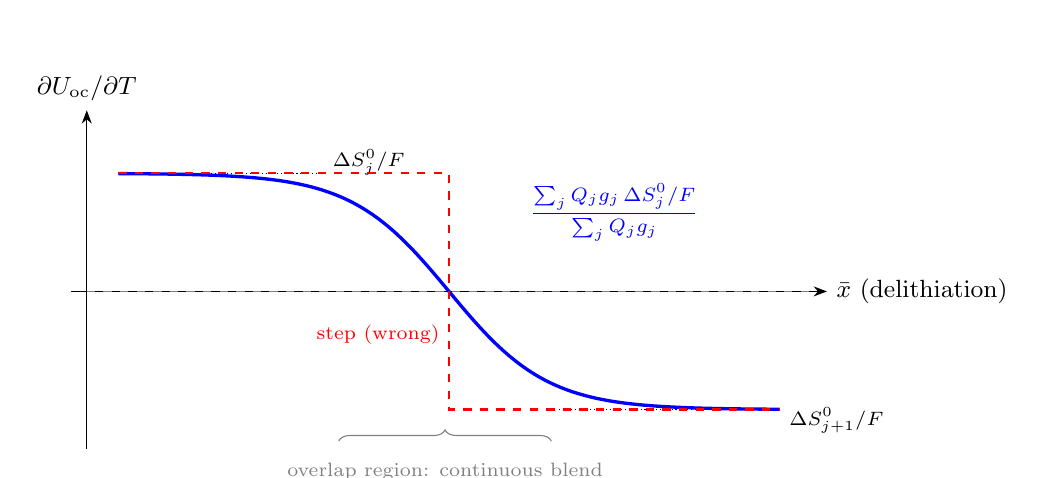
\begin{tikzpicture}[x=1.0cm,y=1.0cm]
  % axes
  \draw[->,>=Stealth] (-0.2,0) -- (9.4,0) node[right]{\small $\bar x$ (delithiation)};
  \draw[->,>=Stealth] (0,-2.0) -- (0,2.3) node[above]{\small $\partial U_\oc/\partial T$};
  \draw[dashed,gray] (0,0) -- (9.2,0);
  % two transition levels dS_j/F (arbitrary units): j has +1.5, j+1 has -1.5
  \draw[densely dotted] (0.4,1.5) -- (3.0,1.5) node[right,black,yshift=4pt]{\scriptsize $\Delta S^0_{j}/F$};
  \draw[densely dotted] (6.0,-1.5) -- (8.8,-1.5) node[right,black,yshift=-4pt]{\scriptsize $\Delta S^0_{j+1}/F$};
  % continuous blend curve: smooth sigmoid from +1.5 to -1.5 centered at x=4.6
  \draw[very thick,blue] plot[smooth,domain=0.4:8.8,samples=80]
    (\x, {1.5 - 3.0/(1+exp(-1.6*(\x-4.6)))});
  % the overlap region shading
  \draw[decorate,decoration={brace,amplitude=4pt},gray] (3.2,-1.9) -- (5.9,-1.9);
  \node[gray,below] at (4.55,-2.05) {\scriptsize overlap region: continuous blend};
  % weight ratio annotation
  \node[blue] at (6.7,1.0) {\scriptsize $\dfrac{\sum_j Q_jg_j\,\Delta S^0_j/F}{\sum_j Q_jg_j}$};
  % NOT a step: contrast dashed step
  \draw[red,dashed,thick] (0.4,1.5) -- (4.6,1.5) -- (4.6,-1.5) -- (8.8,-1.5);
  \node[red] at (3.7,-0.55) {\scriptsize step (wrong)};
\end{tikzpicture}
\caption{겹침 가중식~\eqref{eq:weighted} 이 만드는 \emph{연속 블렌드}(파란 실선): $\bar x$ 가 전이 $j$ 에서 $j{+}1$ 로 넘어갈 때 $\partial U_\oc/\partial T$ 가 $\Delta S^0_j/F$ 에서 $\Delta S^0_{j+1}/F$ 로 국소 $dQ/dV$ 비중 $Q_jg_j/\sum Q_kg_k$ 에 따라 \emph{연속}으로 이동한다. 계단(빨간 점선)이 아니다 — 수치 검증에서 내부 전이 경계 3 곳 모두 연속임이 확인됐다 \cite{numverif2026}. (모식 — 부호$\cdot$하강 순서는 임의다; 흑연 실제 프로파일은 탈리튬화 진행에서 $-16\to-5\to0\to+29$ 로 \emph{상승} 방향, 표~\ref{tab:ds}.)}
\label{fig:blend}
\end{figure}

\subsection{파생 B — 봉우리 내부 configurational 과 이중계산 분리}
완전식이 유한차분값과 정확히 일치하는 이유는, \S\ref{sec:config} 에서 유도한 부분몰 config 항이 정확히 빠진
``단순식의 잔차''이기 때문이다. 단일 전이가 지배하는 영역에서 식~\eqref{eq:dVdT_config} 가 그대로 살아난다:
\begin{equation}
\frac{\partial U_\oc}{\partial T}(x)\;\approx\;\frac{\Delta S_{\rxn,j}}{F}\;+\;\frac{n_jR}{F}\ln\!\frac{\xi_j}{1-\xi_j}
\qquad(\text{단일 전이 지배}).
\label{eq:single_config}
\end{equation}
여기서 두 항이 별개 출처임을 다시 확인한다(파생 B): $\Delta S^0_j/F$ 는 봉우리 \emph{중심}($\xi_j=\tfrac12$,
config$=0$)의 표준값, $n_jR\ln[\xi_j/(1-\xi_j)]/F$ 는 봉우리 \emph{내부}의 분포 항이다. 수치 검증에서 ``완전식
$-$ 단순식'' 차이가 바로 이 config 항이었고(부호 있는 크기 $[-0.21,+0.14]$ mV/K), 이는 \S\ref{sec:config} 의
$+(1/F)\partial S_\config/\partial\theta|_{\theta=1-\xi}$ 와 같은 식이다. \textbf{config 를 $\Delta S^0_j$ 에 또 더하면
이중계산}이며, 올바른 분해는 ``중심 표준값 $+$ 분포 config''로 정확히 한 번씩 센다. 봉우리 중심에서 config$=0$
이므로 두 정의가 모순 없이 맞물린다.

\subsection{파생 C — 폭 $w$ 의 이중지위: 단상 평형 예측 vs.\ 두-상 현상학적 피팅 폭}\label{ssec:weff}
앞 두 파생(A$\cdot$B)은 봉우리 폭 $w_j$ 를 \emph{주어진 입력}으로 받아 모양을 닫았다. 그 $w_j$ 자체를 정하는
것은 전이 종류이며, 이 \emph{이중지위}가 본 절의 전부다.
\begin{itemize}[leftmargin=1.4em,itemsep=2pt]
\item \textbf{단상($\Omega\le2RT$, 균질 고용체)}: 평형 등온선~\eqref{eq:Veq_BW} 이 단조이고, 봉우리 폭은 평형이
\emph{예측}하는 \emph{검증 가능한} 양이다 — 이상 극한에서 $w=RT/F$(상호작용이 있으면 $\Omega$ 가 중심 기울기를 비틀어 폭을
바꾸지만, 그 값 역시 평형 등온선이 결정한다).
\item \textbf{두-상($\Omega>2RT$, 상분리; 흑연 staging 의 두-상 전이 $2\mathrm L\!\to\!2\cdot2\!\to\!1$ 가 여기 속함)}: 평형 \emph{단일 입자}의 등온선은
plateau \emph{안에서} 거의 \emph{델타}(한 전위에 집중)다 — 평형은 폭을 거의 0 으로 예측한다. 그런데 \emph{실측}
$dQ/dV$ 봉우리는 유한 폭의 \emph{종}이며, 이 폭은 평형이 정하는 양이 \emph{아니라} 다음 세 broadening 출처가
정하는 \emph{현상학적 자유 피팅 파라미터}다: (i) 유한 율속의 비대칭 꼬리(단일 입자라도 유한 전류면 표면 SOC
가 평형을 뒤따라 과전압 $\eta$ 가 봉우리를 한쪽으로 민다), (ii) 평탄역 가장자리의 내재 단상 폭($\sim RT/F$,
전류 무관), (iii) 집합 다입자 통계역학 — 전극은 입자 \emph{앙상블}이고, 입자마다 겉보기 전위 apparent-$U=U_j+\eta$ 가
분포($\rho(U_\app)$, 결정성$\cdot$국소환경 차에서 오는 \emph{비-크기} heterogeneity)하여 평형 델타를 종으로
편다. \textbf{이 broadening 의 상세 물리(세 출처의 분해$\cdot$앙상블 forward 통계평균$\cdot$역산 금지$\cdot$입자
크기 효과 배제)는 Chapter 1 의 broadening 절에서 전개하며, 본 장은 그 결과만 받아 $w_j$ 의 \emph{지위}를
규정한다.}
\end{itemize}
따라서 Chapter 2 종합식(\S\ref{sec:revheat})에 들어가는 $w_j$ 는, 흑연 두-상 전이에 대해 평형 예측
$nRT/F$ 를 그대로 믿을 값이 아니라 \emph{다온도 $dQ/dV$ 피팅으로 얻는 현상학적 자유 폭}이다. 임계
$\Omega=2RT$ 의 \emph{열역학}(상분리 plateau 의 발생)은 \S\ref{ssec:BW}$\cdot$\S\ref{sec:limits} 가 다루고, 그
plateau 가 실측에서 \emph{유한 종}이 되는 까닭(=폭의 기원)은 위 broadening 이 다룬다 — 둘은 다른 질문이다.
\begin{warnbox}
\textbf{$w$ 는 종의 폭이지 ``상호작용이 좁힌 델타''가 아니다} — 두-상 실측 봉우리는 평형 델타에서 broadening 으로
\emph{넓어진} 종이므로(좁아진 것이 아니다), ``상호작용 $\Omega$ 가 봉우리를 좁혀 델타로 만든다''는 서술은
\emph{실측 방향과 반대}이며 본 장은 그런 유효-폭 축소식을 쓰지 않는다. $\Omega$ 의 역할은 plateau(상분리)를
\emph{만드는} 임계 조건이며(\S\ref{ssec:BW}), 그 plateau 위의 \emph{유한 폭}은 평형이 아니라 현상학적 피팅이
정한다. (상호작용 엔트로피 $\propto\partial\Omega/\partial T$ 같은 2차 항이 있을 수 있으나, 흑연에서 소수이고
본 장 범위 밖이다.)
\end{warnbox}

\subsection{파생 D — 히스테리시스: 충/방전 분기와 가역/비가역 분리}\label{ssec:hys}
흑연 OCV(open circuit voltage)는 충방전 사이 경로의존이다(준안정 stacking, stage II 무질서) \cite{hysteresis2018}. 분기별 전이 중심을
$U_j^{(d)}=U_j+\tfrac12\sigma_d\,\Delta U_j^\hys$ 로 두면 — $\sigma_d$ 는 탈리튬화 부호(Chapter 1 eq:Ubranch 의
$\gamma_jh_{\eta,j}{=}1$ 특수형)라 흑연 라벨에서 \emph{dis 가 $+\tfrac12$(위 가지), ch 가 $-\tfrac12$(아래 가지)}다 —
각 분기의 엔트로피 계수는 \emph{그 분기의} 봉우리 모양 $g_j^{(d)}$ 로 가중된 \eqref{eq:weighted} 다:
\begin{equation}
\frac{\partial U_\oc^{(d)}}{\partial T}
\;=\;\frac1F\,\frac{\sum_j Q_j\,g_j^{(d)}(x)\,\Delta S_{\rxn,j}}{\sum_j Q_j\,g_j^{(d)}(x)}.
\label{eq:hys_branch}
\end{equation}
가역 발열에 들어가는 것은 두 분기의 \emph{평균}이다 — 충방전을 한 사이클 돌면 히스 중심이 상쇄되고 열역학적
$\Delta S$ 만 남기 때문이다:
\begin{equation}
\boxed{\;\frac{\partial U_\oc^\rev}{\partial T}
\;=\;\tfrac12\Bigl(\frac{\partial U_\oc^\mathrm{ch}}{\partial T}+\frac{\partial U_\oc^\mathrm{dis}}{\partial T}\Bigr)\;.}
\label{eq:hys_rev}
\end{equation}
이 상쇄는 두 분기의 봉우리 형태 $g_j^{(d)}$ 가 같다고 본 \emph{선형화 근사}($\Delta U_j^\hys\!\ll\!w_j$)에서 정확하다.
분기 중심이 서로 달라 같은 $x$ 에서 $g_j^{(\mathrm{ch})}\!\ne\!g_j^{(\mathrm{dis})}$ 이면, 겹침
가중식~\eqref{eq:hys_branch} 의 config 곡률 때문에 평균이 $\Delta S_{\rxn,j}/F$ 로 떨어지는 것은
$\Delta U^\hys$ 의 1차까지이고 유한 $\Delta U^\hys$ 에선 고차 보정이 남는다.
히스 gap $\Delta U^\hys$ 자체는 \emph{비가역} 과정으로, $\propto I\,\Delta U^\hys$ 의 소산율(한 사이클당
$\propto Q_\mathrm{cycle}\,\Delta U^\hys$ 의 소산(entropy production) 열)을 만든다 — 이는 온도 미분 $\partial/\partial T$ 와 \emph{별개}이며 가역열에 섞이지 않는다.
\begin{keybox}
\textbf{혼동 금지.} 가역 발열은 분기 평균~\eqref{eq:hys_rev} 로, 히스 gap 은 비가역열로 \emph{분리} 계산한다.
$\partial U^\rev/\partial T$ 는 분포 재배열의 가역 엔트로피이고, $\Delta U^\hys$ 는 경로 비가역성의 소산이다.
하나의 $\partial U/\partial T$ 로 둘을 뭉뚱그리면 가역/비가역 발열을 섞게 된다(경로의존 측정 불확실도의
정량은 본 장 범위 밖, 공백으로 명시 \cite{hysteresis2018}).
\end{keybox}

% ====================================================================
\section{극한과 코너(corner case) — 분포 검산과 ``$\Delta S_{\rxn,j}$ 상수'' 근사의 타당성}\label{sec:limits}
% ====================================================================
닫힌식의 신뢰는 극한에서 옳은 물리로 환원되는지로 검산된다. 표~\ref{tab:limits} 는 여섯 코너를 정리한다 —
각각 분포 식이 물리적으로 맞는 값으로 가는지 확인한다.

\begin{table}[t]
\centering\small
\renewcommand{\arraystretch}{1.35}
\caption{$\partial U_\oc/\partial T(x)$ 의 극한$\cdot$코너 검산. 규약: $\xi=$ 탈리튬화 진행률($\xi\to1$ 희박, $\xi\to0$ 만충).}
\label{tab:limits}
\begin{tabular}{l l p{0.46\textwidth}}
\toprule
극한 & $\partial U_\oc/\partial T$ 거동 & 물리$\cdot$검증 \\
\midrule
$\xi\to1$ (희박, Li-poor) & config $\to+\infty$ & 삽입 자리 선택지 폭증; 저-$x$ 큰 양 $\Delta S$($+29$)에 분담 기여(귀속 한정 \S\ref{sec:config}) \\
$\xi\to0$ (만충, Li-rich) & config $\to-\infty$ & 배열 선택지 소멸; 만충 정렬의 음 부분몰 엔트로피 \\
$\xi=\tfrac12$ (봉우리 중심) & $=\Delta S_{\rxn,j}/F$ & config$=0$; 중심 표준값 정확 회수(파생 B 일관) \\
$\Omega\to2RT$ (임계) & 상분리 임계(plateau) & $\Omega>2RT$ 측에서 평형 등온선 비단조화$\to$plateau; \emph{실측} 두-상 폭은 현상학적 피팅(\S\ref{ssec:weff}) \\
단일 봉우리 (겹침 0) & $=\Delta S_{\rxn,j}/F+$ config & 가중식~\eqref{eq:weighted} 이 단일 전이로 환원 \\
고온 ($\kB T\!\sim\!E_F$ 근접) & electronic $\propto T$ 우세화 & Fermi--Dirac--Sommerfeld~\eqref{eq:Se} 는 축퇴 극한 $\kB T\!\ll\!E_F$ 전용 — \emph{정성적} 방향(전자 기여 증대)만 유효, $\kB T\!\sim\!E_F$ 에선 정량 부적용 \\
\bottomrule
\end{tabular}
\end{table}

다섯 코너에서 분포 식이 옳은 극한으로 환원되고, 여섯째(고온) 코너는 닫힌식의 적용 한계를 명시한다.
특히 세 가지가 본 장의 골격을 닫는다: (i) 중심
$\xi=\tfrac12$ 에서 config$=0$ 이라 파생 B 의 분리가 자기일관적이다; (ii) 단일
봉우리 한계에서 가중식이 단일 전이 $+$ config 로 환원되므로 \eqref{eq:weighted} 가 \eqref{eq:single_config} 를
포함한다; (iii) $\Omega\to2RT$ 에서 평형 등온선이 비단조로 뒤집혀 상분리 plateau 가 발생하므로, 상호작용 모형이
상전이 임계를 스스로 짚는다.

\begin{keybox}
★\textbf{``$\Delta S_{\rxn,j}$ 전이당 상수'' 근사의 판정.} 측정 $\partial U_\oc/\partial T(x)$ 의 비선형은 두
출처에서 \emph{자동 생성}된다 — (i) 겹침 가중(\S\ref{ssec:overlap})과 (ii) 봉우리 내부 config 분포
(\S\ref{sec:config}). 따라서 $\Delta S_{\rxn,j}(x)$ 를 임의 함수로 둘 필요가 \emph{없다}: 전이당 \emph{상수}
표준값 $+$ 분포만으로 측정급 곡선이 나온다. 이 근사는 \emph{중심 표준값(vib$+$electronic 중심)이 전이 폭 안에서
천천히 변할 때} 타당하다. 예외는 그 항이 전이 폭 \emph{안에서} 급변하는 경우 — 대표적으로 LCO 의 MIT 가 한
전이 안에서 $g(E_F)$ 를 급변시키면 $\Delta S_e(x)$ 만은 $x$-의존으로 유지해야 한다(\S\ref{ssec:elec}). 흑연
하프셀에서는 electronic 이 소수라 이 예외가 거의 없고, config$+$중심 상수로 충분하다.
\end{keybox}

% ====================================================================
\section{가역 발열 — 분포를 재배열하는 열}\label{sec:revheat}
% ====================================================================
이제 분포에서 세운 $\partial U_\oc/\partial T(x)$ 를 가역 발열로 닫는다. 전지 셀의 발열은 Bernardi--Pawlikowski--
Newman 의 일반 에너지 수지 \cite{bernardi1985} 에서 가역(엔트로피)과 비가역(소산) 두 성분으로 갈린다. 단일
활물질 한계에서
\begin{equation}
\dot Q \;=\; \underbrace{I\,(U_\oc-V)}_{\dot Q_\irr\ge0}\;-\;\underbrace{I\,T\,\frac{\partial U_\oc}{\partial T}}_{\dot Q_\rev},
\qquad
\boxed{\;\dot Q_\rev \;=\; -\,I\,T\,\frac{\partial U_\oc}{\partial T}\;=\;-\,\frac{I\,T}{F}\,\Delta S(x)\;,}
\label{eq:qrev}
\end{equation}
이다($I>0$ 방전, $V$ 단자 전압, $U_\oc$ 평형 전위); 첫 항은 과전압 소산(2법칙상 항상 발열, Chapter 1 의
동역학 꼬리$\cdot$분극이 만드는 소산)이고, 둘째 항이 가역열로 부호 양방향이다. 이 축약에는 두 전제가
더 들어 있다 — Bernardi 원식의 혼합 엔탈피(농도 구배 완화열) 항은 준평형 저율(농도 균일)을, 상변화 항은
staging 열이 평형 $U_\oc(x)$ 에 이미 흡수되어 있음을 전제로 소거한 것이며, 전제가 깨지는 고율
조건에서는 두 성분 분해에 잔여 항이 남는다.
★라벨 층위 주의 — 여기서 ``방전($I>0$)''은 Bernardi 셀-수지 관례의 \emph{전기화학적 셀 방전}(자발 방향
$V<U_\oc$, $\dot Q_\irr\ge0$ 이 강제), 곧 흑연 하프셀에선 작동전극의 \emph{리튬화}다. Chapter 1 의 방향
라벨(흑연 하프셀 방전 $=$ 탈리튬화, $\sigma_d{=}+1$)과 같은 단어가 \emph{반대 화학 방향}을 가리키므로,
본 절의 부호는 라벨이 아니라 전류 부호 $I$ 로 읽는다(충전은 $I<0$ 으로 자동 처리 — 식은 방향에 선형).
\begin{srcbox}
부호 규약: 평형 전위와 반응 깁스 에너지가 $\Delta G=-FU_\oc$ 로 묶이고 $\Delta S=-\partial(\Delta G)/\partial T
=+F\,\partial U_\oc/\partial T$ 이므로, 이를 대입하면 식~\eqref{eq:qrev} 의 부호와 정확히 일치한다 \cite{newman,msmr_partI}. 본 장은 평형 전위 $U_\oc$ 기준 $\Delta S=+F\,\partial U_\oc/\partial T$ 규약으로 통일한다(전셀 조립 시 음극 몫은 부호 반전 $+IT\,\partial U_\mathrm{an}/\partial T$ 로 들어가나 본 장 범위 밖 — 상단 범위 박스 참조).
\end{srcbox}

식~\eqref{eq:qrev} 의 $\Delta S(x)$ 는 본 장이 세운 세 분포의 합이므로(\S\ref{sec:vibel} 핵심 박스), 가역
발열은 한 충전상태에서 다른 충전상태로 넘어갈 때 \emph{Li 배열 분포$\cdot$포논 분포$\cdot$전자 분포를 재배열하며
주고받는 열}이다. 부호는 식~\eqref{eq:qrev} 가 곧장 정한다 — 방전($I>0$)에서 $\Delta S>0$ 이면 $\dot Q_\rev<0$ 으로
\emph{흡열}(endothermic, 셀이 열을 흡수), $\Delta S<0$ 이면 $\dot Q_\rev>0$ 으로 \emph{발열}(exothermic)이다($\Delta S$
는 Li 1몰(전자 1몰) 삽입 기준 J\,mol$^{-1}$K$^{-1}$). SOC 에 따라 $\Delta S(x)$ 의 부호가 바뀌므로 흡$\cdot$발열이 교대한다: 저-$x$ 에서
config 양의 발산이 지배해 $\Delta S>0$ 이므로 방전 시 $\dot Q_\rev<0$(흡열), 고-$x$ 에서 vibrational 음
baseline 이 드러나 $\Delta S<0$ 이 되어 방전이 발열로 돈다. stage $2\to1$($x\approx0.5$)의 큰 음의 $\Delta S$
는 방전 시 $\dot Q_\rev>0$, 곧 가역 발열의 두드러진 신호를 남기며, 이는 calorimetry 의 가역 발열 직접 관측과
정합한다 \cite{standardised2024}.

\begin{keybox}
\textbf{계산용 종합식(use-this).} 하프셀 가역 발열을 실제로 산출할 때는 겹침 가중(단순식)에 봉우리 내부 분포
config 를 더한 \emph{완전식}을 쓴다:
\[
\boxed{\;\frac{\partial U_\oc}{\partial T}(x)
=\frac{\sum_j Q_j\,g_j(x)\,\bigl[\Delta S^0_j/F+(n_jR/F)\ln(\xi_j/(1-\xi_j))\bigr]}{\sum_j Q_j\,g_j(x)},\quad
g_j=\frac{\xi_j(1-\xi_j)}{w_j}\;}
\]
$\dot Q_\rev=-IT\,\partial U_\oc/\partial T$ 로 얻으며, \emph{입력}은 $\{\Delta S^0_j,\,Q_j,\,U_j,\,w_j\}$ 와 Chapter 1 의
$\xi_j(V,T)$(본 장 식~\eqref{eq:logistic} — Chapter 1 eq:xieq 에서 $\sigma_d\to s{=}+1$·평형 중심 $U_j$(분기 shift 無)로 둔 형)다. 여기서 $\Delta S^0_j\equiv\Delta S_{\rxn,j}$ 는 봉우리 중심 표준값(파생 B 의
정의)이고, $w_j$ 는 전이별 폭이다(단상 = 평형 예측, 이상 극한 $w_j{=}RT/F$; 흑연 두-상 = 다온도 $dQ/dV$
피팅의 현상학적 자유 폭 — 파생 C \S\ref{ssec:weff}). 지배 두-상 전이($2\mathrm L\!\to\!2\cdot2\!\to\!1$)에서는 완전식의
config 항이 폭의 열적 서식 $w_j=n_jRT/F$ 를 전제하므로, 실측 $w_j$ 가 $T$-동결에 가까우면 완전식 대 단순식의
우열이 $\sim$0.3 mV/K 급으로 뒤집힌다(파생 A srcbox \S\ref{ssec:overlap}) — 지배 두-상 전이의 config 기여는
다온도 round-trip 으로 확정할 대상이며, 그 전까지 단순식(중심값)이 보수적 기준이다. 주어진 탈리튬화 분율 $\bar x$(식~\eqref{eq:implicit} 좌표)에서 $\xi_j$ 를 평가하려면 먼저 전하 보존
음함수~\eqref{eq:implicit} $\sum_j Q_j\xi_{\eq,j}(U_\oc,T)=Q\bar x$ 를 풀어 $U_\oc$ 를 얻고, 그 $U_\oc$ 를
$\xi_j(V,T)$ 에 되먹인다. $\Delta S^0_j$ 는 다온도 $dQ/dV$ 동시 피팅으로 얻고 나머지는 Chapter 1 모수이며, 단일 전이 지배 영역에서 이 식은
식~\eqref{eq:single_config} 로 환원된다.
\end{keybox}

\subsection{계산 예제 — stage $2\!\to\!1$ 부근 한 점의 가역 발열}\label{ssec:worked}
종합식이 실제로 한 수를 내는 과정을 Chapter 1 의 4-전이 staging 파라미터(중심 $U_j$$\cdot$용량 $Q_j$$\cdot$중심 표준
엔트로피 $\Delta S^0_j$[표~\ref{tab:ds}], 폭은 다중도 $n_j{=}1$ 의 열적 폭 $w_j{=}RT/F\!\approx\!25.7$ mV)로 한 SOC 에서
끝까지 따라간다 --- 코드(\texttt{Anode\_Fit\_v1.0.15})가 내는 값 그대로다. 대표점은 탈리튬화 분율 $\bar x=0.25$
($T=298.15$ K) --- stage $2\!\to\!1$($\mathrm{LiC_6}$, 큰 음의 $\Delta S^0=-16$ J\,mol$^{-1}$K$^{-1}$)이 지배하는 저-$\bar x$ 영역이다.

\textbf{(a) 전하 보존으로 $U_\oc$ 결정.} 음함수~\eqref{eq:implicit} $\sum_jQ_j\xi_{\eq,j}(U_\oc,T)=Q\bar x$
($Q=\sum_jQ_j=0.97\,Q_\cell$)를 $U_\oc$ 에 대해 풀면(좌변이 $U_\oc$ 에 단조라 유일근)
\begin{equation*}
U_\oc(\bar x{=}0.25,\,298.15\,\mathrm K)=74.4\ \mathrm{mV}.
\end{equation*}
\textbf{(b) 전이별 진행률과 봉우리 가중.} 이 $U_\oc$ 에서 식~\eqref{eq:logistic} 의
$\xi_{\eq,j}=\{1{+}\exp[-(U_\oc-U_j)/w_j]\}^{-1}$ 과 $g_j=\xi_j(1-\xi_j)/w_j$ 를 전이마다 읽어 표~\ref{tab:worked} 에
모은다. 가중 분모 $\sum_jQ_jg_j=6.18\,Q_\cell$/V 가 곧 그 점의 측정 $dQ/dV$ 이며, 비중이 ``$2\!\to\!1$ 봉우리가
$75\%$ 활성''임을 그대로 읽는다(\S\ref{ssec:overlap}).

\begin{table}[htbp]
\centering\small
\renewcommand{\arraystretch}{1.2}
\caption{계산 예제($\bar x{=}0.25$, $298.15$ K; $w_j{=}RT/F$)의 전이별 중간값 — 진행률 $\xi_j$, 봉우리 가중
$g_j=\xi_j(1-\xi_j)/w_j$, 국소 $dQ/dV$ 비중, 중심 표준 계수 $\Delta S^0_j/F$, 봉우리 내부 config 항 $(n_jR/F)\ln[\xi_j/(1-\xi_j)]$.}
\label{tab:worked}
\begin{tabular}{lccccc}
\toprule
전이 & $\xi_j$ & $g_j$ [V$^{-1}$] & 비중 $Q_jg_j/\!\sum$ & $\Delta S^0_j/F$ [mV/K] & config [mV/K] \\
\midrule
$4\!\to\!3$   & $0.005$ & $0.19$ & $0.003$ & $+0.301$ & $-0.458$ \\
$3\!\to\!2\mathrm L$ & $0.072$ & $2.61$ & $0.051$ & $0.000$ & $-0.220$ \\
$2\mathrm L\!\to\!2$ & $0.143$ & $4.77$ & $0.193$ & $-0.052$ & $-0.154$ \\
$2\!\to\!1$   & $0.395$ & $9.30$ & $0.753$ & $-0.166$ & $-0.037$ \\
\bottomrule
\end{tabular}
\end{table}
\textbf{(c) 겹침 가중 엔트로피 계수(완전식).} 열적 폭 $w_j{=}n_jRT/F$ 라 봉우리 내부 config 항이 살아,
식~\eqref{eq:weighted} 의 완전식(중심값 $+$ config)을 비중으로 가중하면
\begin{equation*}
\begin{aligned}
\frac{\partial U_\oc}{\partial T}
&=\sum_j\frac{Q_jg_j}{\sum_kQ_kg_k}\Big[\frac{\Delta S^0_j}{F}+\frac{n_jR}{F}\ln\frac{\xi_j}{1-\xi_j}\Big]\\
&=0.753(-0.203)+0.193(-0.206)+0.051(-0.220)+0.003(-0.157)
=-0.204\ \mathrm{mV/K}.
\end{aligned}
\end{equation*}
(중심값만 쓴 단순식은 $-0.134$ mV/K 이고, config 항이 $-0.070$ mV/K 를 더한다.)
\textbf{(d) round-trip 실증.} 열적 폭 $w_j{=}n_jRT/F$ 아래 중심 $U_j(T)$ 와 폭 $w_j(T)$ 를 함께 움직여
$U_\oc(\bar x,T)$ 를 $T\pm3$ K 에서 두 번 푼 유한차분 $[U_\oc(T{+}3)-U_\oc(T{-}3)]/6\,\mathrm K$ 는 $-0.204$ mV/K 로,
해석 완전식~\eqref{eq:weighted}과 $<\!0.001\ \mu$V/K 로 일치한다 --- 음함수 미분 사슬(config 항 포함)이 수치와
왕복 정합함을 이 한 점에서 확인한다(전 범위 검증은 파생 A). 코드 \texttt{entropy\_coefficient} 도 같은 $-0.204$ 를 낸다. \textbf{(e) 유효 반응 엔트로피와 가역 발열.} 정의 $\Delta S(\bar x)=F\,\partial U_\oc/\partial T$ 와
Bernardi 출구~\eqref{eq:qrev} $\dot Q_\rev=-IT\,\partial U_\oc/\partial T$ 로 닫으면
\begin{equation*}
\Delta S(\bar x{=}0.25)=-19.7\ \mathrm{J\,mol^{-1}K^{-1}}<0,
\qquad
\frac{\dot Q_\rev}{I}=-T\frac{\partial U_\oc}{\partial T}=+60.8\ \mathrm{mV}\;(=+60.8\ \mathrm{mW/A}).
\end{equation*}
곧 이 SOC 에서 셀 방전($I>0$, 흑연 리튬화)은 $\dot Q_\rev>0$ 의 \emph{발열}이며, stage $2\!\to\!1$ 의 큰 음의
$\Delta S$ 가 남기는 가역 발열 신호(calorimetry 관측 \cite{standardised2024})와 부호$\cdot$규모가 정합한다.
config 항은 폭의 열적 서식 $w_j{=}n_jRT/F$ 를 전제하므로($n_j$ 키 기준), 지배 $2\!\to\!1$ 이 두-상이라 실측 폭이
$T$-동결에 가까우면 config 몫은 다온도 round-trip 으로 확정할 대상이고(use-this 박스$\cdot$\S\ref{ssec:weff}),
그 하한은 단순식 $-0.134$ mV/K 다.

\begin{table}[t]
\centering\small
\renewcommand{\arraystretch}{1.25}
\caption{탈리튬화 진행에 따른 가역 발열의 부호 교대(완전식, 298.15 K; Chapter 1 4-전이 staging, $w_j{=}RT/F$). $\dot Q_\rev/I$ 는
방전($I>0$) 기준 단위 전류당 열이며 $+$ 가 발열이다. 저-$\bar x$(Li-rich, stage $2\!\to\!1$/$2\mathrm L\!\to\!2$
음의 $\Delta S$)는 방전 발열, 고-$\bar x$(Li-poor, config 양의 발산)는 방전 흡열로, 부호가 SOC 를 따라 뒤집힌다.}
\label{tab:qrev}
\begin{tabular}{cccccc}
\toprule
$\bar x$ & $U_\oc$ [mV] & $\partial U_\oc/\partial T$ [mV/K] & $\Delta S$ [J\,mol$^{-1}$K$^{-1}$] & $\dot Q_\rev/I$ [mV] & 방전 열 \\
\midrule
$0.10$ & $43.5$  & $-0.307$ & $-29.6$ & $+91.5$ & 발열 \\
$0.25$ & $74.4$  & $-0.204$ & $-19.7$ & $+60.8$ & 발열 \\
$0.50$ & $109.0$ & $-0.089$ & $-8.6$  & $+26.6$ & 발열 \\
$0.75$ & $148.8$ & $+0.044$ & $+4.3$  & $-13.2$ & 흡열 \\
$0.90$ & $195.2$ & $+0.218$ & $+21.0$ & $-64.9$ & 흡열 \\
\bottomrule
\end{tabular}
\end{table}

표~\ref{tab:qrev} 가 이 계산을 다섯 SOC 로 확장해 \emph{같은 종합식 하나}가 흡$\cdot$발열의 SOC 교대(저-$\bar x$
발열 $\to$ 고-$\bar x$ 흡열)를 자동으로 냄을 보인다 — 임의 함수나 외부 스위치 없이 분포만으로. 한 종합식이
SOC 축을 따라 가역 발열의 부호를 스스로 뒤집는 이 거동이, 본 장이 세운 세 분포가 발열에서 맺는 매듭이다.

\textbf{한계$\cdot$갭(정직).} 본 장의 닫힌식에는 다음 공백이 남는다: (1) 완전식의 표시-정밀도 일치(파생 A,
175 점)는 \emph{시뮬레이션 자기일관성} 검증이다 — 남는 공백은 그 완전식이 가정하는 logistic
전이형$\cdot$파라미터 집합 $\{\Delta S^0_j,Q_j,U_j,w_j\}$ 가 실측 흑연을 얼마나 충실히 재현하는지를
\emph{실데이터 round-trip 피팅}으로 확정하는 일이다(시뮬레이션 검증과 실측 검증의 구분). (2) 히스테리시스 하 경로의존 $\partial U_\oc/\partial T$ 의 측정 불확실도
정량화는 본 장 범위 밖이며, 파생 D(\S\ref{ssec:hys})는 가역/비가역 분리의 틀만 제시한다 \cite{hysteresis2018}. (3) 상호작용
$\Omega$ 의 온도 의존(파생 C 의 2차 항)과 그 흑연에서의 값은 아직 확보하지 못했다. (4) electronic 항의 절대값은
흑연에서 소수로 취급했으며, LCO 의 MIT 예외는 분포 언어의 사례로만 다뤘다. (5) 전셀 합성은 본 장의 범위
밖이고, 그 근거는 서두 범위 박스에 명시했다.

\begin{procedurebox}
\textbf{방법론 출구 — 다온도 $dQ/dV$ 에서 중심 표준값 $\Delta S^0_j=F\,\dd U_j/\dd T$ 추정 절차.} 위 종합식의 입력
$\{\Delta S^0_j,Q_j,U_j,w_j\}$ 중 전이별 중심 표준값 $\Delta S^0_j$ 는 다음 순서로 추정한다.
\begin{enumerate}[leftmargin=1.8em,itemsep=2pt,topsep=2pt]
\item 충분히 낮은 율의 준평형 코인 하프셀 $dQ/dV$ 를 여러 온도 $T_k$ 에서 측정한다(저율$\cdot$과평활 회피로
전이 폭이 동역학 lag 로 부풀지 않게 한다).
\item 측정 전위에서 분극을 먼저 분리한다 — Chapter 1 의 $V_n=V_\mathrm{app}-\sigma_d|I|R_n$ 로 IR$\cdot$과전압을
빼야 \emph{평형} $U_\oc$ 의 온도 의존만 남는다.
\item 같은 $Q_j$ 구조를 공유하되 각 온도의 중심 $U_j(T_k)$ 와 폭 $w_j(T_k)$ 를 허용해 Chapter 1 의 logistic
전이 모델~\eqref{eq:logistic} 을 \emph{동시} 피팅하며, 이는 반응별 $U_j^0(T)$ 를 온도 연속함수로 두는 MSMR
(Multi-Species, Multi-Reaction) 절차와 직접 대응한다 \cite{msmr_partI,msmr_partII}.
\item 회귀한 $U_j(T)$ 의 중심 기울기에서 $\Delta S^0_j=F\,\dd U_j/\dd T$ 를 얻고, Allart 등의 전극 분리
$\Delta S(x)$ \cite{allart2018} 와 부호$\cdot$규모를 대조해 검증한다(표~\ref{tab:ds}).
\item 봉우리 \emph{내부}의 $x$-의존은 따로 입력하지 않는다 — 식~\eqref{eq:single_config} 의 분포 config 항
$(n_jR/F)\ln[\xi_j/(1-\xi_j)]$ 가 자동으로 채우며, 마지막으로 종합식과 $\dot Q_\rev=-IT\,\partial U_\oc/\partial T$
(Bernardi 출구 \cite{bernardi1985})로 가역 발열을 산출한다.
\end{enumerate}
\end{procedurebox}

% ====================================================================
\section*{맺음}
\addcontentsline{toc}{section}{맺음}
% ====================================================================
본 장은 코인 하프셀의 엔트로피와 가역 발열을 \emph{통계열역학}으로 세웠다. 분배함수 $Z$ 에서 점유 분포
$\avg{n}$ 을 끌어내 그것이 Chapter 1 logistic 의 기원임을 보였고($w=RT/F$ 가 분포 폭), 점유 분포에서
configurational 엔트로피와 그 발산하는 부분몰 항을, 같은 분포 언어로 vibrational(포논 Bose--Einstein)$\cdot$electronic
(Fermi--Dirac--Sommerfeld) 엔트로피를 세웠다. 세 분포가 합쳐 측정 $\partial U_\oc/\partial T(x)$ 의 모든 모양을 만든다:
겹침 가중(파생 A, 수치 검증 완료)으로 봉우리 사이 연속 블렌드를, 봉우리 내부 config(파생 B, 이중계산 분리)로
$x$-의존을, 폭 $w_j$ 의 이중지위(파생 C — 단상은 평형 예측, 흑연 두-상은 현상학적 자유 피팅 폭, broadening
기원은 Chapter 1)로 두-상 폭의 지위를, 히스 분기 평균(파생 D)으로 가역/비가역
분리를 닫았다. 극한 여섯 코너가 분포 식을 검산하고, ``전이당 상수 $\Delta S^0_j$ $+$ 분포''로 측정급 비선형이
모델 안에서 자기일관하게 산출됨을 보였다(지배 두-상 전이의 폭 $T$-의존은 다온도 round-trip 으로 확정할 대상).
가역 발열 $\dot Q_\rev=-IT\,\partial U_\oc/\partial T$ 은 이 분포들을 재배열하는 열이다.

% ====================================================================
\begin{thebibliography}{99}
\bibitem{bernardi1985} D. Bernardi, E. Pawlikowski, J. Newman, ``A General Energy Balance for Battery Systems,'' \emph{J. Electrochem. Soc.} \textbf{132}(1), 5--12 (1985). DOI: 10.1149/1.2113792.
\bibitem{newman} J. Newman, K. E. Thomas-Alyea, \emph{Electrochemical Systems}, 3rd ed., Wiley (2004). (OCV($T$): slope $=\Delta S$, intercept $=\Delta H$; lattice-gas insertion thermodynamics.)
\bibitem{huggins2009} R. A. Huggins, \emph{Advanced Batteries: Materials Science Aspects}, Springer (2009). (격자기체 삽입 전극 열역학·Bragg--Williams 평형 전위.)
\bibitem{bazant2013} M. Z. Bazant, ``Theory of Chemical Kinetics and Charge Transfer Based on Nonequilibrium Thermodynamics,'' \emph{Acc. Chem. Res.} \textbf{46}(5), 1144--1160 (2013). DOI: 10.1021/ar300145c. (regular-solution lattice-gas OCV·상분리 임계 $\Omega=2RT$.)
\bibitem{reynier2003} Y. Reynier, R. Yazami, B. Fultz, ``The entropy and enthalpy of lithium intercalation into graphite,'' \emph{J. Power Sources} \textbf{119--121}, 850--855 (2003). DOI: 10.1016/S0378-7753(03)00285-4.
\bibitem{allart2018} D. Allart \emph{et al.}, ``Model of Lithium Intercalation into Graphite by Potentiometric Analysis with Equilibrium and Entropy Change Curves of the Graphite Electrode,'' \emph{J. Electrochem. Soc.} \textbf{165}(2), A380 (2018). DOI: 10.1149/2.1251802jes.
\bibitem{occupation2019} ``Transitions of lithium occupation in graphite: A physically informed model in the dilute lithium occupation limit supported by electrochemical and thermodynamic measurements,'' \emph{Electrochimica Acta} (2019). DOI: 10.1016/j.electacta.2019.135634. [방법 수준 인용 — 원문 식 미확보.]
\bibitem{chemmater2015} ``Intercalation Compounds from LiH and Graphite: Relative Stability of Metastable Stages\ldots,'' \emph{Chem. Mater.} \textbf{27} (2015). DOI: 10.1021/acs.chemmater.5b00235. [형성 ΔH calorimetry — abstract tier.]
\bibitem{jpcc2021} ``Thermodynamic Analysis of Li-Intercalated Graphite by First-Principles Calculations with Vibrational and Configurational Contributions,'' \emph{J. Phys. Chem. C} \textbf{125}(51) (2021). DOI: 10.1021/acs.jpcc.1c08992. [abstract tier.]
\bibitem{msmr_partI} ``Quantifying the Entropy and Enthalpy of Insertion Materials for Battery Applications Via the Multi-Species, Multi-Reaction Model,'' \emph{J. Electrochem. Soc.} (2024). DOI: 10.1149/1945-7111/ad1d27. [Chapter 1 이 인용하는 ECS Advances 의 ``Part 1''(MCMB 흑연 파라미터화, DOI: 10.1149/2754-2734/ad7d1c)과는 \emph{별개 논문} — 두 문헌이 공유하는 것은 Part II(DOI: 10.1149/1945-7111/ad70d9) 뿐이다.]
\bibitem{msmr_partII} ``Quantifying the Temperature Dependence of the MSMR Model Part II: Estimation of Entropy Coefficient for Meso-Carbon Micro-Bead Graphite,'' \emph{J. Electrochem. Soc.} (2024). DOI: 10.1149/1945-7111/ad70d9.
\bibitem{standardised2024} ``A Standardised Potentiometric Method for the Effective Parameterisation of Reversible Heating in a Lithium-Ion Cell,'' \emph{J. Electrochem. Soc.} (2024). DOI: 10.1149/1945-7111/ad4918.
\bibitem{hysteresis2018} ``Uncertainties in entropy due to temperature path dependent voltage hysteresis in Li-ion cells,'' \emph{J. Power Sources} (2018). DOI: 10.1016/j.jpowsour.2018.05.060.
\bibitem{numverif2026} 본 연구 내부 수치 검증(Derivative A), \texttt{Anode\_Fit\_v1.0.15} 4-전이 흑연 staging 파라미터, 유한차분 vs.\ 가중식 비교 (2026). [내부 자료 — 표시 정밀도 일치 PASS, 본문 \S\ref{ssec:overlap} 요지.]
\end{thebibliography}

\end{document}
